%% Source: https://github.com/tias/constraint-solving-course
%% Licensed under CC BY-NC-SA 4.0: https://creativecommons.org/licenses/by-nc-sa/4.0/
%% You may share and adapt this for non-commercial use,
%% with attribution and under the same license.

\documentclass{cons-beamer}

\begin{document}


\begin{frame}{L02: Basic Modeling} %: variables, constraints (&functions) and objectives}
  \begin{center}
    ~ \\
    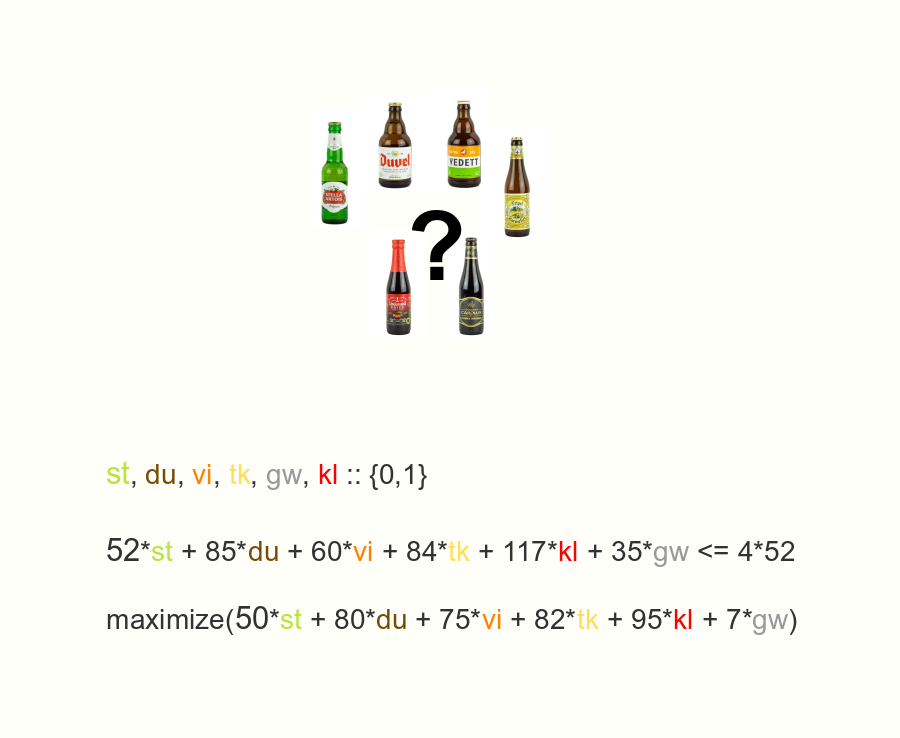
\includegraphics[height=42mm]{images/beer_taste_prob.png} \\
    Prof. Tias Guns and Dr. Dimos Tsouros \\[0.5em]
    
\includegraphics[width=2cm]{images/kuleuven_CMYK_logo.pdf}
  \end{center}
  
  {\footnotesize 
  Partly based on slides from Pierre Flener, Uppsala University.}
  % https://pierre-flener.github.io/courses/M4CO/lectures.html
\end{frame}


\section{Recap: combinatorial problem to solution}

\begin{frame}{Combinatorial Optimisation}
  \begin{center}
    \begin{tabular}{c c} % 2-column grid for images
      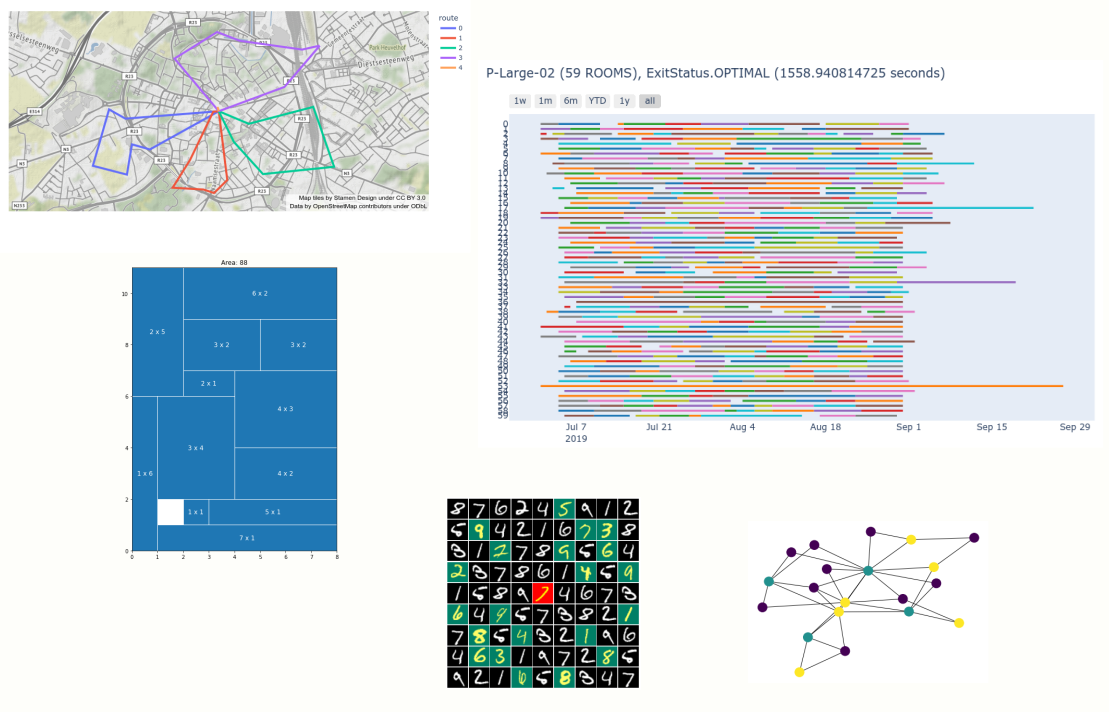
\includegraphics[height=40mm]{images/CO_examples} &
        
\includegraphics[width=20mm]{images/physicians} 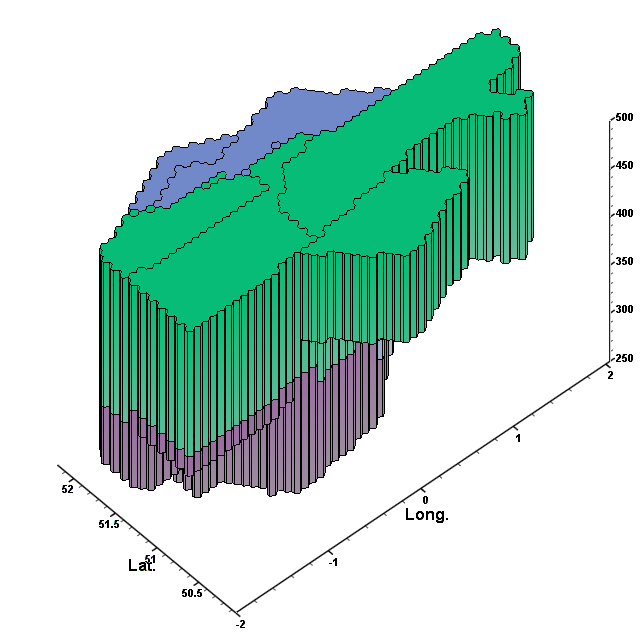
\includegraphics[height=20mm]{images/sectorLondon} \\
      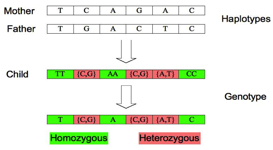
\includegraphics[height=20mm]{images/genotype-haplotype} &
        
\includegraphics[height=20mm]{images/burningLaptop}
    \end{tabular}
  \end{center}
\end{frame}

\begin{frame}{Model-and-Solve}
  \centering
  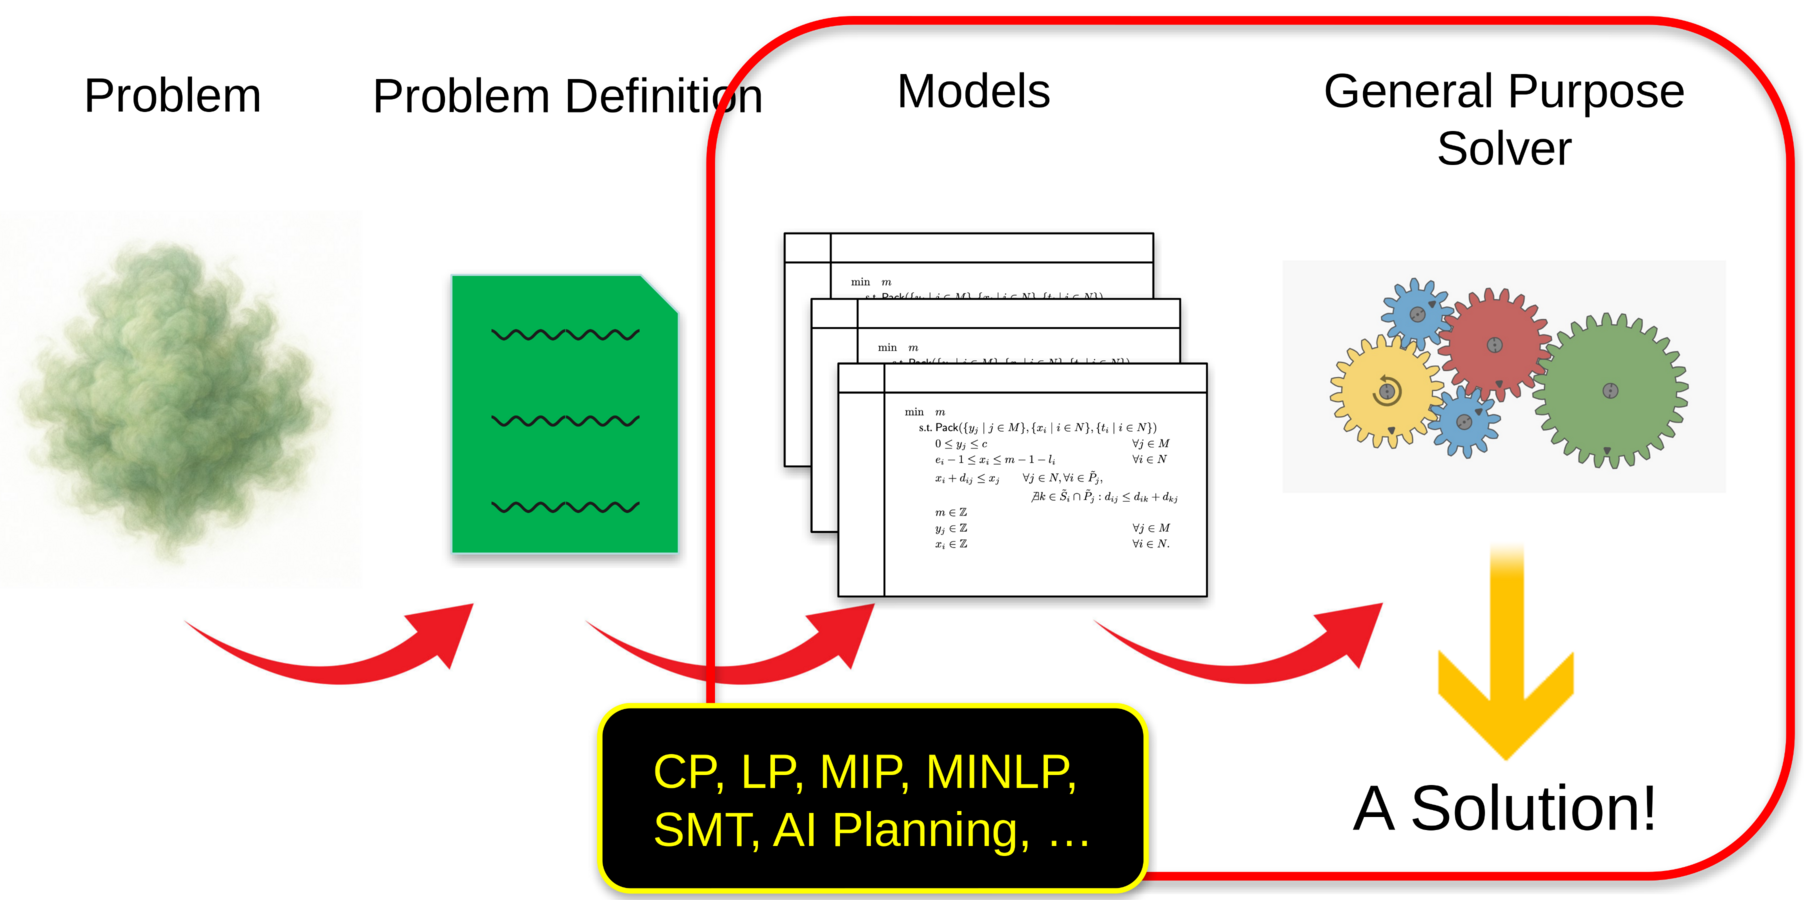
\includegraphics[height=68mm]{images/prob2sol}
\end{frame}

\begin{frame}{Modelling (declarative) vs Programming (imperative)}
  \begin{center}
    \begin{tikzpicture}
      [->,>=stealth',level/.style={level distance=20mm,sibling distance=50mm}]
      \tikzset{nod/.style = {font=\bfseries}}
      \node[nod, align=center](problem){Problem \\ \normalfont\textit{(multi-eyed beast)}}
      child{
        node[nod, align=center](def){Problem Definition \\ \normalfont\textit{(free form, unambiguous)}}
        child{
          node[nod, align=center]{Model \\ \normalfont\textit{(formal specification)}}
          child{
            node[nod]{program}
            edge from parent node[left] {automatic!}
          }
          edge from parent node[above left, yshift=-8pt] {\underline{what?} }
        }
        child{
          node[nod, align=center]{Algorithm \\ \normalfont\textit{(pseudo-code)}}
          child{
            node[nod]{program}
            edge from parent node[right] {manual!}
          }
          edge from parent node[above right, yshift=-8pt] {\underline{how?} }
        }
      };
    \end{tikzpicture}
  \end{center}
\end{frame}

\begin{frame}%{An example problem definition \& model}
  \begin{example}[Problem Definition: Sudoku]
    The goal of Sudoku is to \textit{complete} a partially filled 9x9 grid with numbers so that each row, column and 3x3 section contains each digit between 1 and 9 once.
  \end{example}
  
  \begin{example}[Model: Sudoku]
    \vspace{-1em}
    \begin{align*}
      &G_{ij} \in \{1, 2, \ldots, 9\} & \quad\quad &\forall i, j \in \{1, \ldots, 9\} \\
      &\cons{AllDifferent}{\{G_{ij} | j \in \{1, \ldots, 9\}\}} & \quad\quad & \forall i \in \{1, \ldots, 9\} \\
      &\cons{AllDifferent}{\{G_{ij} | i \in \{1, \ldots, 9\}\}} & \quad\quad & \forall j \in \{1, \ldots, 9\} \\
      &\cons{AllDifferent}{\{G_{kl} | k \in \{i, \ldots, i+2\},  l \in \{j, \ldots, j+2\}\}} & \quad\quad & \forall i,j \in \{1, 4, 7\} \\
      &G_{ij} = v & \quad\quad & \forall (i,j,v) \in {\cal D}
    \end{align*}
  \end{example}
\end{frame}

\begin{flashcardcpmpy}
\begin{frame}%{An example problem definition \& model}
  \begin{example}[Problem Definition: Sudoku]
    The goal of Sudoku is to \textit{complete} a partially filled 9x9 grid with numbers so that each row, column and 3x3 section contains each digit between 1 and 9 once.
  \end{example}

  \begin{example}[Model: Sudoku in CPMpy]
    \vspace{-0.5em}
    \lstinputlisting[language=cpmpy,firstline=17,lastline=27]{models_cpmpy/T01_sudoku.py}
    \vspace{-0.5em}
  \end{example}
\end{frame}
\end{flashcardcpmpy}

\begin{frame}
\frametitle{From Model to Model to Solver}

\begin{tikzpicture}[scale=0.8, every node/.style={transform shape}, node distance=0.5cm]

% Model (green box)
\node[draw, fill=green!30, rounded corners, minimum width=2cm, minimum height=1cm] (model) {Model  (high-level modelling language)};

% Decompose-globals (blue box)
\node[draw, fill=blue!20, below=of model, rounded corners, minimum width=3.5cm, minimum height=1cm] (decompose) {decompose globals};
% Flatten (orange box)
\node[draw, fill=blue!20, below=of decompose, rounded corners, minimum width=3.5cm, minimum height=1cm] (flatten) {flatten};
% Linearize (purple box)
\node[draw, fill=blue!20, below=of flatten, rounded corners, minimum width=3.5cm, minimum height=1cm] (linearize) {linearize};
% int2bool (cyan box)
\node[draw, fill=blue!20, below=of linearize, rounded corners, minimum width=3.5cm, minimum height=1cm] (int2bool) {int to bool};
% pb2sat (pink box)
\node[draw, fill=blue!20, below=of int2bool, rounded corners, minimum width=3.5cm, minimum height=1cm] (pb2sat) {pb to sat};

% Low-level mdoels (no fill)
\node[draw, fill=green!30, rounded corners, dotted, minimum height=1cm, minimum width=4cm, right=1cm of decompose, align=left] (smt) {SMT model};
\node[draw, fill=green!30, rounded corners, dotted, minimum height=1cm, minimum width=4cm, right=1cm of flatten, align=left] (cp) {CP model};
\node[draw, fill=green!30, rounded corners, dotted, minimum width=4cm, right=1cm of linearize, fill=green!30, rounded corners, align=left] (ilp) {ILP model};
\node[draw, fill=green!30, rounded corners, dotted, minimum height=1cm, minimum width=4cm, right=1cm of int2bool, align=left] (pb) {PB model};
\node[draw, fill=green!30, rounded corners, dotted, minimum height=1cm, minimum width=4cm, right=1cm of pb2sat, align=left] (sat) {(max)SAT model};

% Solvers (no fill)
\node[draw, minimum height=1cm, minimum width=4cm, right=1cm of smt, align=left] (smt2) {SMT solver};
\node[draw, minimum height=1cm, minimum width=4cm, right=1cm of cp, align=left] (cp2) {CP solver};
\node[draw, minimum height=1cm, minimum width=4cm, right=1cm of ilp, align=left] (ilp2) {ILP solver};
\node[draw, minimum height=1cm, minimum width=4cm, right=1cm of pb, align=left] (pb2) {PB solver};
\node[draw, minimum height=1cm, minimum width=4cm, right=1cm of sat, align=left] (sat2) {(max)SAT solver};

% Arrows
\draw[->] (model) -- (decompose); 
\draw[->] (decompose) -- (flatten);
\draw[->] (flatten) -- (linearize);
\draw[->] (linearize) -- (int2bool);
\draw[->] (int2bool) -- (pb2sat);

% Connections to low-level
\draw[->] (decompose.east) -- ++(0.5,0) |- (smt.west);
\draw[->] (flatten.east) -- ++(0.5,0) |- (cp.west);
\draw[->] (linearize.east) -- ++(0.5,0) |- (ilp.west);
\draw[->] (int2bool.east) -- ++(0.5,0) |- (pb.west);
\draw[->] (pb2sat.east) -- ++(0.5,0) |- (sat.west);

% Connections to solvers
\draw[->] (smt.east) -- ++(0.5,0) |- (smt2.west);
\draw[->] (cp.east) -- ++(0.5,0) |- (cp2.west);
\draw[->] (ilp.east) -- ++(0.5,0) |- (ilp2.west);
\draw[->] (pb.east) -- ++(0.5,0) |- (pb2.west);
\draw[->] (sat.east) -- ++(0.5,0) |- (sat2.west);

\end{tikzpicture}

\end{frame}


\begin{frame}[fragile]{High-level vs low-level modelling languages}

  High-level modeling languages (CPMpy, MiniZinc, Essence)

  \begin{itemize}
    \item Model = list of \textit{complex} expressions over decision variables
    \item Boolean logic example: (symbols are explained later) \\
          $(a \leftrightarrow (b \vee (c \wedge d))) \wedge (e \vee \neg f)$
  \end{itemize} \vfill

  Low-level modeling language (SAT, ILP, CP, ...)

  \begin{itemize}
    \item Model = list of \textit{atomic} constraints over decision variables
    \item SAT: CNF Example: $(a \vee \neg b) \wedge (a \vee \neg n) \wedge (\neg a \vee b \vee n) \wedge (n \vee \neg c \vee \neg d) \wedge (\neg n \vee c) \wedge (\neg n \vee d) \wedge (e \vee \neg f)$
  \end{itemize} \vfill

  Typically, high-level languages can translate to multiple low-level languages \textit{(solver-agnostic)}.
  \vfill

  This course uses 1 high-level language, all ideas translate to other languages and to low-level languages.
\end{frame}

\begin{frame}{So what does solving do?}
  For a CP solver, a model = list of \textit{atomic} constraints over decision variables.
  
  \begin{center}
    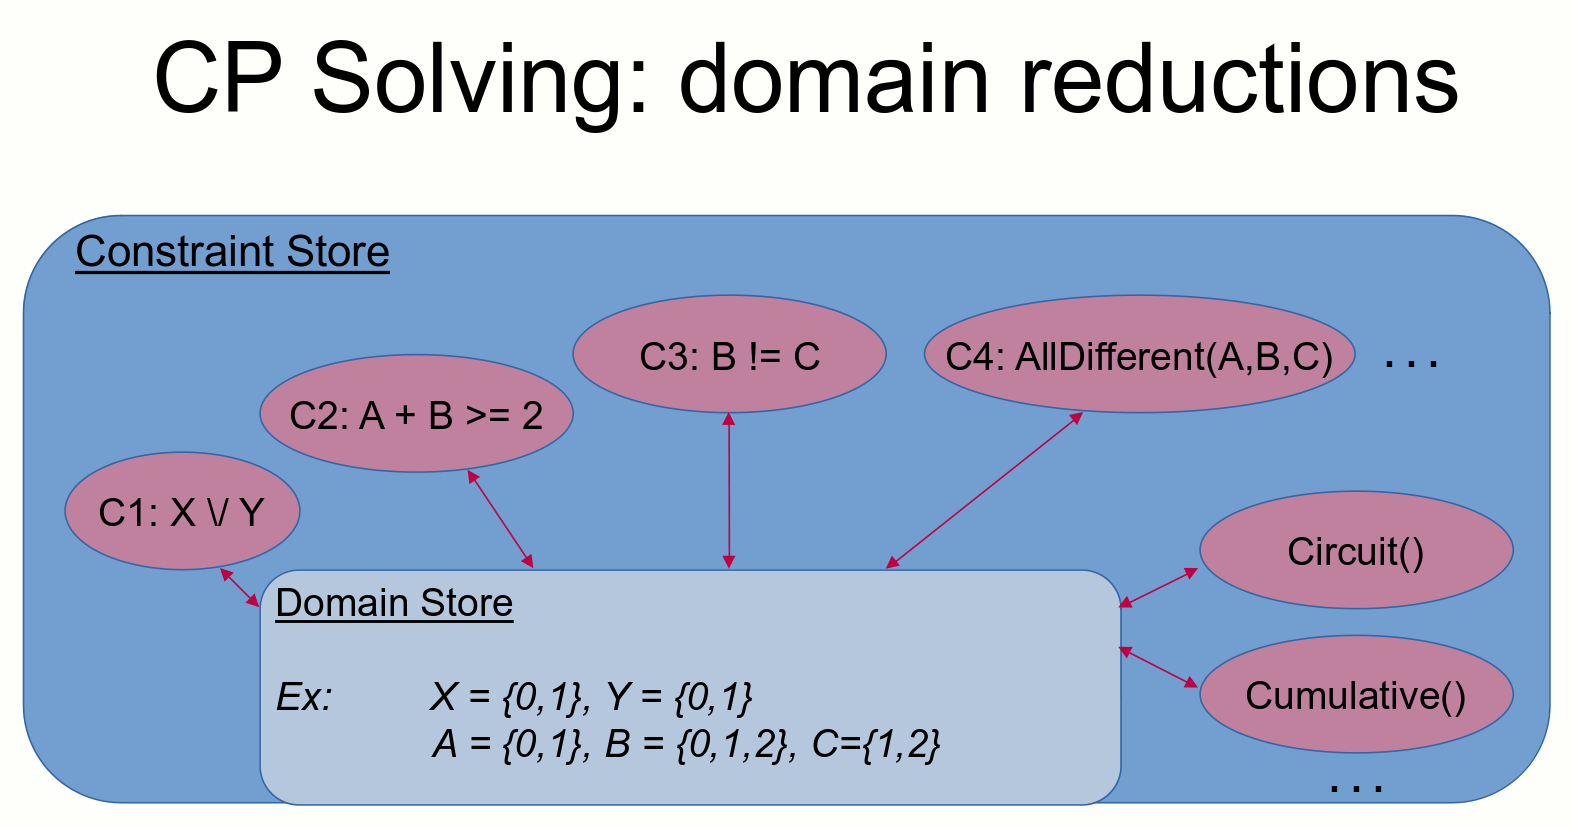
\includegraphics[height=48mm, trim=0 0 0 50mm, clip]{images/constraint_store} % cut top title
  \end{center}
  
  It will iterate over the constraints and try to reduce domains (=propagation) \\
  and branch over variables if there is nothing left to reduce (=search)
\end{frame}

\begin{frame}{Branching induces a search tree}
  \vfill
  
% Reduced Search Space with Constraints
\scriptsize	
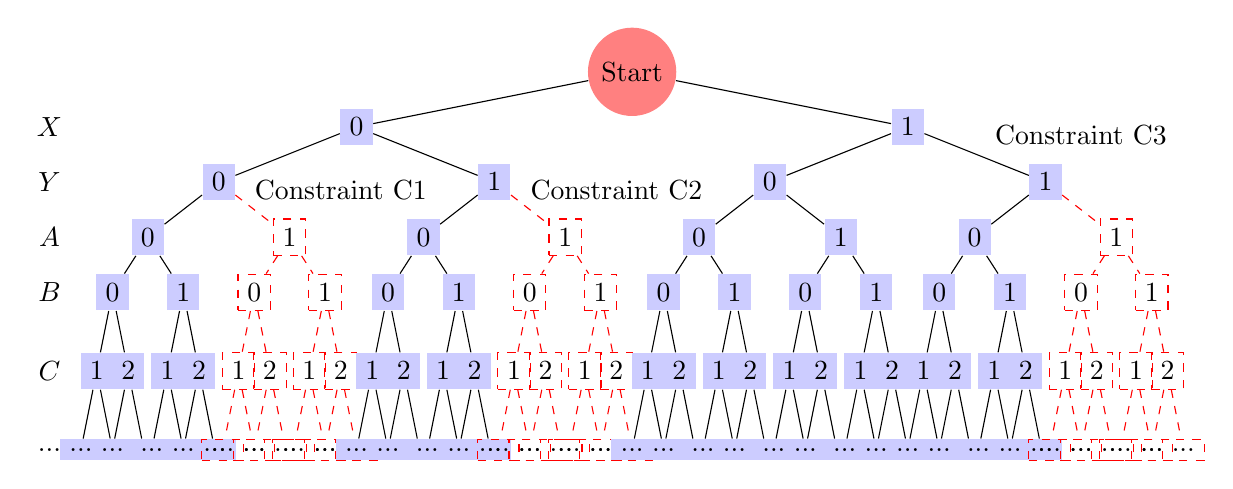
\begin{tikzpicture}[
val/.style={rectangle, fill=blue!20},
root/.style={circle, fill=red!50},
var/.style={rectangle},
pruned/.style={rectangle, draw=red, dashed},
level 1/.style={level distance=0.7cm, sibling distance=7cm},
level 2/.style={level distance=0.7cm, sibling distance=3.5cm},
level 3/.style={level distance=0.7cm, sibling distance=1.8cm},
level 4/.style={level distance=0.7cm, sibling distance=0.9cm},
level 5/.style={level distance=1cm, sibling distance=0.4cm},
]

% Variables listed on the side
\coordinate (V) at (-7.4,0);
\node[var] at (V) { };
\coordinate (A) at (-7.4,-0.7);
\node[var] at (A) {$X$};
\coordinate (B) at (-7.4,-1.4);
\node[var] at (B) {$Y$};
\coordinate (C) at (-7.4,-2.1);
\node[var] at (C) {$A$};
\coordinate (D) at (-7.4,-2.8);
\node[var] at (D) {$B$};
\coordinate (E) at (-7.4,-3.8);
\node[var] at (E) {$C$};
\coordinate (E) at (-7.4,-4.8);
\node[var] at (E) {...};

% Root node and expanded search space with values only
\node[root] {Start} 
  child{node[val]{0} % X=0
    child{node[val]{0} % Y=0
      child{node[val]{0} % A=0
        child{node[val]{0} % B=0
          child{node[val]{1}
           child{node[val]{...}}
           child{node[val]{...}}           
           } % C=1
          child{node[val]{2}
           child{node[val]{...}}
           child{node[val]{...}}  
           } % C=2
        }
        child{node[val]{1} % B=1
          child{node[val]{1}
         child{node[val]{...}}
           child{node[val]{...}}
           } % C=1
          child{node[val]{2}
           child{node[val]{...}}
           child{node[val]{...}}  
           } % C=2
        }
      }
      child[pruned]{node[pruned]{1} % A=1
        child[pruned]{node[pruned]{0} % B=0
          child[pruned]{node[pruned]{1}
           child[pruned]{node[pruned]{...}}
           child[pruned]{node[pruned]{...}}           
           } % E=1
          child[pruned]{node[pruned]{2}
           child[pruned]{node[pruned]{...}}
           child[pruned]{node[pruned]{...}}  
           } % E=2
        }
        child[pruned]{node[pruned]{1} % B=1
          child[pruned]{node[pruned]{1}
           child[pruned]{node[pruned]{...}}
           child[pruned]{node[pruned]{...}}           
           } % E=1
          child[pruned]{node[pruned]{2}
           child[pruned]{node[pruned]{...}}
           child[pruned]{node[pruned]{...}}  
           } % E=2
        }
      }
    }
    child{node[val]{1} % Y=1
      child{node[val]{0} % A=0
        child{node[val]{0} % B=0
          child{node[val]{1}
           child{node[val]{...}}
           child{node[val]{...}}           
           } % C=1
          child{node[val]{2}
           child{node[val]{...}}
           child{node[val]{...}}  
           } % C=2
        }
        child{node[val]{1} % B=1
          child{node[val]{1}
           child{node[val]{...}}
           child{node[val]{...}}           
           } % C=1
          child{node[val]{2}
           child{node[val]{...}}
           child{node[val]{...}}  
           } % C=2
        }
      }
      child[pruned]{node[pruned]{1} % A=1
        child[pruned]{node[pruned]{0} % B=0
          child[pruned]{node[pruned]{1}
           child[pruned]{node[pruned]{...}}
           child[pruned]{node[pruned]{...}}           
           } % C=1
          child[pruned]{node[pruned]{2}
           child[pruned]{node[pruned]{...}}
           child[pruned]{node[pruned]{...}}  
           } % C=2
        }
        child[pruned]{node[pruned]{1} % B=1
          child[pruned]{node[pruned]{1}
           child[pruned]{node[pruned]{...}}
           child[pruned]{node[pruned]{...}}           
           } % C=1
          child[pruned]{node[pruned]{2}
           child[pruned]{node[pruned]{...}}
           child[pruned]{node[pruned]{...}}  
           } % C=2
        }
      }
    }
  }
  child{node[val]{1} % X=1
    child{node[val]{0} % Y=0
      child{node[val]{0} % A=0
        child{node[val]{0} % B=0
          child{node[val]{1}
           child{node[val]{...}}
           child{node[val]{...}}           
           } % C=1
          child{node[val]{2}
           child{node[val]{...}}
           child{node[val]{...}}  
           } % C=2
        }
        child{node[val]{1} % B=1
          child{node[val]{1}
         child{node[val]{...}}
           child{node[val]{...}}
           } % C=1
          child{node[val]{2}
           child{node[val]{...}}
           child{node[val]{...}}  
           } % C=2
        }
      }
      child{node[val]{1} % A=1
        child{node[val]{0} % B=0
          child{node[val]{1}
           child{node[val]{...}}
           child{node[val]{...}}           
           } % C=1
          child{node[val]{2}
           child{node[val]{...}}
           child{node[val]{...}}  
           } % C=2
        }
        child{node[val]{1} % B=1
          child{node[val]{1}
         child{node[val]{...}}
           child{node[val]{...}}
           } % C=1
          child{node[val]{2}
           child{node[val]{...}}
           child{node[val]{...}}  
           } % C=2
        }
      }
    }
    child{node[val]{1} % Y=1
      child{node[val]{0} % A=0
        child{node[val]{0} % B=0
          child{node[val]{1}
           child{node[val]{...}}
           child{node[val]{...}}           
           } % C=1
          child{node[val]{2}
           child{node[val]{...}}
           child{node[val]{...}}  
           } % C=2
        }
        child{node[val]{1} % B=1
          child{node[val]{1}
           child{node[val]{...}}
           child{node[val]{...}}           
           } % C=1
          child{node[val]{2}
           child{node[val]{...}}
           child{node[val]{...}}  
           } % C=2
        }
      }
      child[pruned]{node[pruned]{1} % A=1
        child[pruned]{node[pruned]{0} % B=0
          child[pruned]{node[pruned]{1}
           child[pruned]{node[pruned]{...}}
           child[pruned]{node[pruned]{...}}           
           } % C=1
          child[pruned]{node[pruned]{2}
           child[pruned]{node[pruned]{...}}
           child[pruned]{node[pruned]{...}}  
           } % C=2
        }
        child[pruned]{node[pruned]{1} % B=1
          child[pruned]{node[pruned]{1}
           child[pruned]{node[pruned]{...}}
           child[pruned]{node[pruned]{...}}           
           } % C=1
          child[pruned]{node[pruned]{2}
           child[pruned]{node[pruned]{...}}
           child[pruned]{node[pruned]{...}}  
           } % C=2
        }
      }
    }
  };

% Labels for pruned branches
\node at (-3.7, -1.5) {\inference{Constraint C1}};
\node at (-0.2, -1.5) {\inference{Constraint C2}};
\node at (5.7, -0.8) {\inference{Constraint C3}};

\end{tikzpicture}

\end{frame}


\section{Modeling basics}

\subsection{Basic example}

% Its just a knapsack problem, but grounded in Belgium's beer culture,
% which should be drank responsibly (as the example demonstrates)
\begin{frame}{Belgian Beer Tasting problem}

  $ $\\
  Responsible drinking:\\
  What beers to try, so that you can still pay attention in class tomorrow?

  \begin{center}
    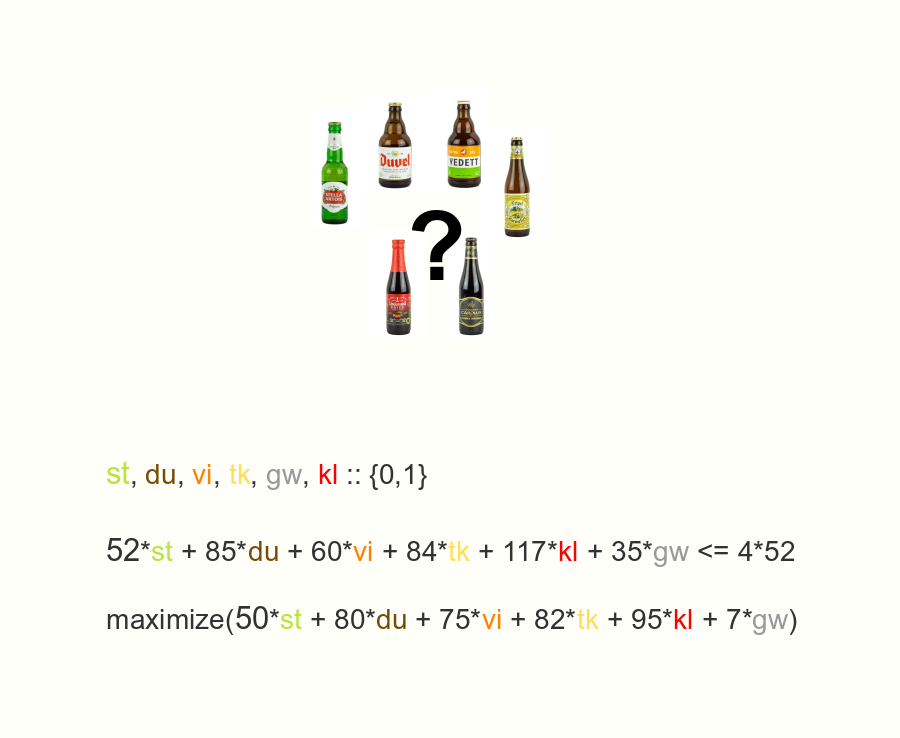
\includegraphics[height=62mm, trim=0 100mm 0 0, clip]{images/beer_taste_prob.png}
  \end{center}
\end{frame}

\begin{frame}
  \centering
  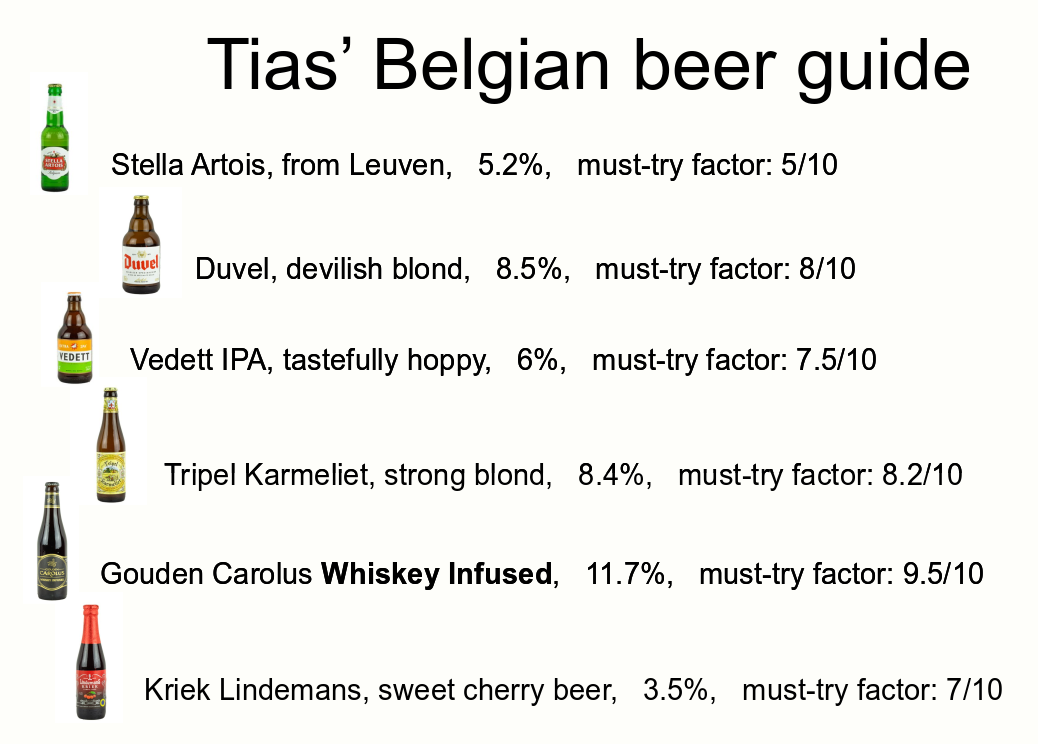
\includegraphics[height=82mm]{images/beer_guide.png}
\end{frame}

\begin{frame}{Belgian Beer Tasting problem}
  
  \begin{columns}
    \begin{column}{0.35\textwidth}
      What beers to try, so that you can still pay attention in class tomorrow? \\[2em]
      \textbf{Model =} \\[1em]
      - Variables, with a domain \\[1em]
      - Constraints over variables \\[1em]
      - Optionally: an objective \\[2em]
      \textbf{Model.solve()} \\[2em]
    \end{column}
    \begin{column}{0.65\textwidth}
      {\vspace{-2.5em}
      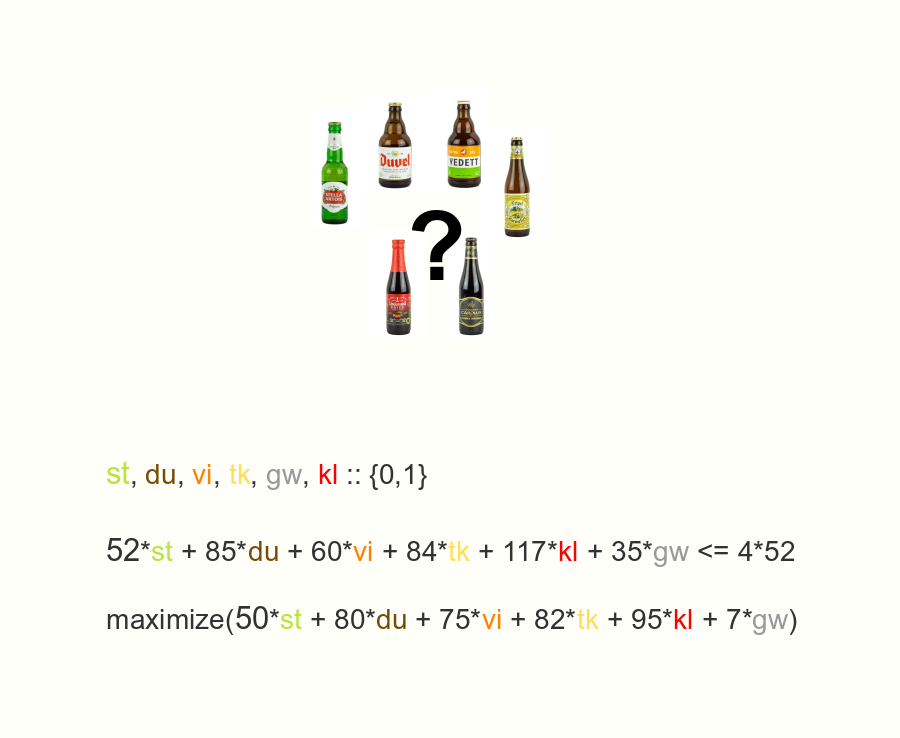
\includegraphics[height=25mm, trim=0 100mm 0 30mm, clip]{images/beer_taste_prob.png}}

        
      \textcolor{green}{st}, \textcolor{orange}{du}, \textcolor{purple}{vi}, \textcolor{brown}{tk}, \textcolor{gray}{gc}, \textcolor{red}{kl} $\in$ \{0,1\} \\[1em]

        
      {\small 52*\textcolor{green}{st} + 85*\textcolor{orange}{du} + 60*\textcolor{purple}{vi} + 84*\textcolor{brown}{tk} + 117*\textcolor{gray}{gc} + 35*\textcolor{red}{kl} $\leq$ 4*52} \\[1em]

        
      {\small maximize(50*\textcolor{green}{st} + 80*\textcolor{orange}{du} + 75*\textcolor{purple}{vi} + 82*\textcolor{brown}{tk} + 95*\textcolor{gray}{gc} + 70*\textcolor{red}{kl})}
    \end{column}
  \end{columns}
\end{frame}

\begin{flashcardcpmpy}
\begin{frame}[fragile]{Belgian Beer Tasting problem, CPMpy}
  \begin{columns}
    \begin{column}{0.35\textwidth}
      What beers to try, so that you can still pay attention in class tomorrow? \\[2em]
      \textbf{Model =} \\[1em]
      - Variables, with a domain \\[1em]
      - Constraints over variables \\[1em]
      - Optionally: an objective \\[2em]
      \textbf{Model.solve()} \\[2em]
    \end{column}
    \begin{column}{0.65\textwidth}
      $ $\\[5.2em]
      \lstinputlisting[language=cpmpy, firstline=1, lastline=11]{models_cpmpy/T02_beer_tasting.py}
    \end{column}
  \end{columns}
\end{frame}
\end{flashcardcpmpy}


\subsection{Decision variables}

\begin{frame}{Decision variables}
  In this course, we only consider \defined{discrete decision variables}, namely Boolean and integer decision variables:

  \begin{align}
    b &\in \{0,1\} \\
    x &\in \{1, \ldots, 10\}
  \end{align}

  \vspace{1em}
  Variables have a \defined{domain}, a finite set of allowed values:
  \begin{itemize}
    \item for {Boolean} variables, this is always $\{0,1\}$
    \item for {integer} variables, this is specified as two parameters: \\
    \textit{lb}=lower bound, \textit{ub}=upper bound, domain: $\{lb..ub\}$
  \end{itemize}

  \vspace{1em}
  Sometimes, you want to create a variable with a \defined{sparse domain}: $x \in \{1,2,5,8,9\}$

  \vspace{1em}
  Some modeling languages support other variables (floats, sets, strings, bitvectors)
\end{frame}


\subsection{Logical constraints}

\begin{frame}{Logical constraints}

  $ $\\
  Logical constraints involve Boolean operators over Boolean expressions

  $ $\\
  Boolean operators:

  $ $\\
  \begin{itemize}
    \item negation: $\neg a$ \quad(in text sometimes $-a$)
    \item or: $a \vee b$ \quad(in text sometimes written as $a\mid b$)
    \item and: $a \wedge b$ \quad(in text sometimes written as $a~\&~b$)
    \item equivalence: $a \leftrightarrow b$ \quad(also called \defined{reification} or double-implication)
    \item implication: $a \rightarrow b$ \quad(also called \defined{half-reification})
  \end{itemize}

  $ $\\
  Each operator has its own \textit{truth table}: a/b values that make the expression true or false.
\end{frame}

\begin{frame}{Logical constraints}

  Each operator has its own \textit{truth table}: a/b values that make the expression true or false.

  $ $\\
  The one many people find tricky is the one of \textbf{implication}, called \defined{material implication} in logic:
  {%\footnotesize
  \begin{center}
  \begin{tabular}{|c|c|c|}
    \hline
    $a$ & $b$ & $a \rightarrow b$ \\
    \hline
    T & T & T \\
    T & F & F \\
    F & T & T \\
    F & F & T \\
    \hline
  \end{tabular}
  \end{center}
  }

  $ $\\
  Verify: $a \rightarrow b$ is equivalent to $\neg a \vee b$\\
  Also: $a = b$ is equivalent to $(a \rightarrow b) \wedge (b \rightarrow a)$

\end{frame}

\begin{frame}{Logical constraints}
  $ $\\
  Boolean quantifiers:

  $ $\\
  \begin{itemize}
    \item universal quantification: $\forall x \in X, (x \rightarrow y)$
    \item existential quantification: $\exists x \in X, (x \wedge y)$
  \end{itemize}

  $ $\\
  Other Boolean operator:

  \begin{itemize}
    \item exclusive-or: $a \otimes b$ \quad(in text sometimes $a ~\mbox{xor}~ b$)
  \end{itemize}

  \begin{center}
    \begin{tabular}{|c|c|c|}
      \hline
      \( a \) & \( b \) & \( a \otimes b \) \\
      \hline
      T & T & F \\
      T & F & T \\
      F & T & T \\
      F & F & F \\
      \hline
    \end{tabular}
  \end{center}

  $ $\\
  To think about: $a \otimes b$ is equivalent to $(a \vee b) \wedge (\neg a \vee \neg b)$, what about $\mbox{XOR}(a,b,c)$?
\end{frame}


\subsection{Simple comparison constraints}

\begin{frame}{Simple comparison constraints}

  $ $\\
  Simple comparisons ($=, \neq, <, \leq, >, \geq)$ of an integer variable:

  \begin{align}
      x &= 3 \\
      y &\neq 6 \\
      z & < 2
  \end{align}

  $ $\\
  A simple comparison is a Boolean-valued expression, it can be used inside Boolean operators:
  \begin{align}
      &(x = 3) \wedge (y > 5) \\
      &(y \neq 6) \rightarrow (a \vee (z < 2))
  \end{align}
  Good use of brackets () avoids ambiguity.
\end{frame}


\subsection{Arithmetic constraints}

\begin{frame}{Arithmetic constraints}

  Arithmetic constraints combine arithmetic operations $(+,-,*,/)$ over integers with a comparisons ($=, \neq, <, \leq, >, \geq)$:

  \begin{align}
    x + y &= 3 \\
    y - z &\neq 6 \\
    2*z - (x*y + y) & < 2
  \end{align}

  $ $\\
  Integer division $x/y == 5$ is tricky because it is undefined for $y=0$. It is a \defined{partial function}. Some languages/systems simply forbid a division where the nominator has $0$ in its domain.

  (there are more peculiarities with integer division, such as using \textit{floor division} or \textit{rounding division} for negative numbers...)
\end{frame}

\begin{frame}{Arithmetic constraints}

  Linear constraints only involve arithmetic operations $(+, -)$ and a multiplication of a variable with a constant. \defined{Linear inequalities} further only use the comparisons $(<, \leq, >, \geq)$:

  \begin{align}
    x + y &\geq 3 \\
    y - z &< 6 + x
  \end{align}

  $ $\\
  All integer linear inequalities can be rewritten to a normal form $a_1x_1 + \ldots + a_n x_n \leq b$

  $ $\\
  A linear equality $x + y = 5$ can be rewritten as $(x + y \leq 5) \wedge (x + y \geq 5)$

  $ $\\
  A linear dis-equality $x + y \neq 5$ leads to a disjunction: $(x + y < 5) \vee (x + y > 5)$ and cannot be rewritten to a conjunction of inequalities without adding a new variable...

\end{frame}

\begin{frame}{Arithmetic constraints}
  Many other arithmetic operations exist:

  \begin{itemize}
    \item absolute value $|a|$
    \item modulo $x \% y$
    \item minimum $min(x,y,z)$
    \item maximum $max(x,y,z)$
  \end{itemize}

  $ $\\
  These can be used in arithmetic constraints too (e.g. arithmetic operators + comparison).

  $ $\\
  Just like simple constraints, arithmetic constraints are Boolean-valued expressions too; and can be used in Boolean expressions.

  $ $\\
  A \defined{nested expression} nests all sorts of Boolean operators and/or arithmetic constraints and operators. A contrived example: $(a \vee (|x - y| > z/2)) \rightarrow (r * s \neq  max(x, y-t, |z-3|)) \wedge (b \otimes (c \leftrightarrow  d))$

\end{frame}


\subsection{Global constraints}

\begin{frame}{Global constraints}

  $ $\\
  Many other constraints and operations that do not exist in standard mathematics can be defined.

  In the constraint programming community, such constraints are called \defined{global constraints}:

  \begin{itemize}
    \item AllDifferent$(x, y, z)$
    \item Table$([x,y], [[1,2],[1,4],[3,4]])$
    \item Count$(X, 3) == z$
    \item ...
  \end{itemize}

  In some systems, the concept 'Count$(X, 3) == z$' is modelled with a predicate 'Count$(X, 3, z)$'.

  In this course, we call the 'Count$(X, 3)$' part a \defined{global function}, the integer-valued counter-part of a global constraint; such that it can be nested with arithmetic operators, e.g. $10*(Count(X, 3) - Count(Y, 3))$
\end{frame}


\subsection{Objective functions}

\begin{frame}{Objective functions}

  $ $\\
  The \defined{objective function} is an integer-valued expression that must be minimized or maximized.

  $ $\\
  \textit{Global functions} are valid integer-valued expressions too, as are nested arithmetic expressions (in high-level languages at least).

  $ $\\
  Sometimes, we want to relax a hard constraint by allowing it to be violated, but penalizing that \textbf{violation in the objective}.

  When we add a constraint (Boolean-valued expression) to the objective function, we call that constraint a \defined{soft constraint}, e.g. $\Iverson{z == 0}$ below:

  \vspace{-1em}
  {\footnotesize
  \begin{align}
    \mbox{maximize} \quad&10*x + 3*y + \Iverson{z == 0} \\
    \mbox{s.t.} \quad &x + y < 10, \\
                &x + y + z > 5, \\
                &x, y, z \in \{0..10\}
  \end{align}
  }
\end{frame}


% THIS ENTIRE PART IS CPMPY SPECIFIC, and hence in flashcard environment
% We will repeat each of the previous subsections, but with language syntax details
\begin{flashcardcpmpy}
\section{Modelling with the CPMpy library}

\begin{frame}
  \begin{columns}[T] % align columns at the top
    \begin{column}{0.5\textwidth} % left column
      \vspace*{5em}
      Using CPMpy includes the following:
      \begin{itemize}
        \item Import and model creation
        \item Decision variables
        \item Constraints
        \item Objective function (optional)
        \item Solving
        \item Printing output
      \end{itemize}
    \end{column}
    \begin{column}{0.5\textwidth} % right column
      \begin{example}[Showcase]
        \vspace{-0.5em}
        \lstinputlisting[language=cpmpy]{models_cpmpy/T02_showcase.py}
      \end{example}
    \end{column}
  \end{columns}
\end{frame}

\begin{frame}{Install, import, create model}
  Single page, all you need documentation: 
  \url{https://cpmpy.readthedocs.io/en/latest/modeling.html}

  \vspace{2em}
  Installing:
  \lstinline[basicstyle=\scriptsize\ttfamily]$pip install cpmpy$

  \vspace{2em}
  Importing and model creation:
  \lstinputlisting[language=cpmpy,firstline=1,lastline=2]{models_cpmpy/T02_showcase.py}

  \vspace{2em}
  \footnotesize
  You can also \lstinline[language=cpmpy]{from cpmpy import *} which will override any/all/min/max/sum for convenience but this can be confusing for novices (e.g. when does \cpminline{sum} compute a value or create an expression).
\end{frame}

\begin{frame}{Decision variables}
  CPMpy supports \defined{discrete decision variables}, namely Boolean and integer decision variables:

  \lstinputlisting[language=cpmpy,firstline=3,lastline=4]{models_cpmpy/T02_decisvars.py}

  \vspace{1em}
  Variables have a \defined{domain}, a finite set of allowed values:
  \begin{itemize}
    \item for {Boolean} variables, this is implicitely $\{0,1\}$
    \item for {integer} variables, this is specified as the first two parameters: \\
    \textit{lb}=lower bound, \textit{ub}=upper bound, domain: $\{lb..ub\}$
  \end{itemize}

  \vspace{1em}
  If you want a \defined{sparse domain}, containing only a few values, you can:
  \begin{itemize}
      \item Add constraints to forbid specific values, e.g. \lstinline[language=cpmpy]{x != 3, x != 5, x != 7}
      \item Or use the shorthand \textit{InDomain} global constraint: \lstinline[language=cpmpy]{cp.InDomain(x, [1,2,4,6,8,9])}
  \end{itemize}
\end{frame}

\begin{frame}{Decision variables 2/2}
  Decision variables have a unique \defined{name}. You can set it yourself, otherwise a unique name will automatically be assigned to it. If you print decision variables, \lstinline[language=cpmpy]{print(b, x)}, it will print the name.

  \vspace{1em}
  CPMpy creates \emph{n-dimensional} \defined{NumPy arrays} when creating variables!

  This is very convenient for Numpy-style \emph{vectorized} operations and for integration with machine learning libraries.

  \vspace{1em}
  The \emph{shape} argument allows you to specify the dimensions of the array. All variables will have the same initial domain:
  \lstinputlisting[language=cpmpy,firstline=6,lastline=11]{models_cpmpy/T02_decisvars.py}
\end{frame}

\begin{frame}{Note: Numpy indexing}
  Python creates lists of lists, each requiring an index:
  \lstinputlisting[language=cpmpy,firstline=4,lastline=6]{models_cpmpy/T02_indexing.py}

  Numpy creates an array, which allows indexing with a tuple:
  \lstinputlisting[language=cpmpy,firstline=8,lastline=9]{models_cpmpy/T02_indexing.py}

  Also accepts `:` which means this entire dimension:
  \lstinputlisting[language=cpmpy,firstline=11,lastline=11]{models_cpmpy/T02_indexing.py}

  Or using an equal sized array of Booleans (also called a 'selector'):
  \lstinputlisting[language=cpmpy,firstline=13,lastline=15]{models_cpmpy/T02_indexing.py}
\end{frame}

\begin{frame}{Advanced: Vectorized operations}
  Because decision variables are NumPy arrays in CPMpy, you can also do \defined{vectorized operations} on them: an operation on two equal sized arrays will create an (equal sized) array of element-wise operations:

  \begin{example}[vectorized operations]
    \vspace{-0.5em}
    \lstinputlisting[language=cpmpy,firstline=3,lastline=6]{models_cpmpy/T02_vectorized.py}
    \vspace{-0.5em}
  \end{example}

  \defined{Broadcasting} in NumPy allows operations between arrays of different shapes, by automatically expanding the smaller array along its dimensions to match the larger array's shape: %, enabling element-wise operations without the need for explicit replication of data.

  \begin{example}[broadcasting]
    \vspace{-0.5em}
    \lstinputlisting[language=cpmpy,firstline=8,lastline=8]{models_cpmpy/T02_vectorized.py}
    \vspace{-0.5em}
  \end{example}
\end{frame}

\begin{frame}{Expressing constraints}
  A \defined{constraint} is an expression that is added to a model, the solver will enforce it to always be true, e.g.:

  \lstinputlisting[language=cpmpy,firstline=9,lastline=11]{models_cpmpy/T02_showcase.py}

  The \cpminline{m += O} is Python syntactic sugar for \cpminline{m.__add__(O)}.

  $ $\\
  We will differentiate \emph{Boolean-valued} \defined{expressions} like \lstinline[language=cpmpy]{X[0] == 1} and \textit{integer-valued} expressions like \lstinline[language=cpmpy]{X[1] + X[2]}. Only Boolean-valued expressions can be added as a constraint.

\end{frame}

\begin{frame}{Common constraints}
  \begin{example}[Typical logical constraints]
    \vspace{-0.5em}
    \lstinputlisting[language=cpmpy,firstline=5,lastline=10]{models_cpmpy/T02_constraints.py}
    \vspace{-0.5em}
  \end{example}
  CPMpy overloads the Python bitwise operators \cpminline{&, |, ~}. They have precedence over all other operators, so \cpminline{a == 0 | b == 1} is \textbf{wrongly} interpreted as \cpminline{a == (0 | b) == 1} \texttt{-- WRONG!}. So make sure to \textbf{always write explicit brackets} to express \cpminline{(a == 0) | (b == 1)}.
  \begin{example}[n-ary logical constraints]
    \vspace{-0.5em}
    \lstinputlisting[language=cpmpy,firstline=12,lastline=15]{models_cpmpy/T02_constraints.py}
    \vspace{-0.5em}
  \end{example}
\end{frame}

\begin{frame}{Common constraints 2/4}
  %TODO: have it column-by-column?
  \begin{example}[Typical comparison constraints]
    \vspace{-0.5em}
    \lstinputlisting[language=cpmpy,firstline=17,lastline=25]{models_cpmpy/T02_constraints.py}
    \vspace{-0.5em}
  \end{example}
  You can not use a numeric expression as a Boolean expression, e.g. invalid: \cpminline{b | x} \texttt{-- WRONG!}, you need to add your intended meaning of truth: \cpminline{b | (x != 0)}
\end{frame}

\begin{frame}{Common constraints 3/4}
  %TODO: first show math notation...
  \begin{example}[Some arithmetic constraints]
    \vspace{-0.5em}
    \lstinputlisting[language=cpmpy,firstline=28,lastline=37]{models_cpmpy/T02_constraints.py}
    \vspace{-0.5em}
  \end{example}
  You \textbf{can} use any Boolean expression as a numeric expression, e.g. valid: \cpminline{b + x > 2}
\end{frame}

\begin{frame}{Common constraints 4/4}
  \begin{example}[Typical global constraints]
    \vspace{-0.5em}
    \lstinputlisting[language=cpmpy,firstline=40,lastline=48]{models_cpmpy/T02_constraints.py}
    \vspace{-0.5em}
  \end{example}
  Many more global constraints and global functions exists! We will see them throughout the course.

  \vspace{1em}
  \begin{footnotesize}
    Handy summary sheet: \url{https://cpmpy.readthedocs.io/en/latest/summary.html}

  \end{footnotesize}

\end{frame} 

\begin{frame}{Objective functions (optional)}
  If a model has \textit{no objective function} specified, then it is a \defined{satisfaction problem}: the goal is to find out whether a solution, any solution, exists. 

  When an objective function is added it is an \defined{optimisation problem} and this function needs to be minimized or maximized.

  \begin{example}[Objective function, from showcase example]
    \vspace{-0.5em}
    \lstinputlisting[language=cpmpy,firstline=13,lastline=14]{models_cpmpy/T02_showcase.py}
  \end{example}
  Any expression can be added as an objective function (\cpminline{maximize()} or \cpminline{minimize()})

  \vspace{1em}
  CPMpy does not support multi-objective optimisation yet: \\ multiple
  objective functions must either be aggregated into a weighted sum, \\
  or handled outside the model.
\end{frame}

\begin{frame}{Solving and printing output}
 \begin{example}[Solving]
  \vspace{-0.5em}
  \lstinputlisting[language=cpmpy,firstline=3,lastline=7]{models_cpmpy/T02_solving.py}
  \vspace{-0.5em}
 \end{example}

  solve() accepts arguments such as \cpminline{time_limit=}, \cpminline{solver=} and solver-specific ones

  \begin{example}[Printing output]
    \vspace{-0.5em}
    \lstinputlisting[language=cpmpy,firstline=8]{models_cpmpy/T02_solving.py}
    \vspace{-0.5em}
  \end{example}
\end{frame}

\begin{frame}{Focus point: reification}
  Reification enables the reasoning about the truth of a constraint \\
  or a Boolean expression. \vfill
  \begin{example}
    constraint \cpminline{x < y}\\    
    requires that \cpminline{x} be smaller than \cpminline{y}. \vfill
    constraint \cpminline{b == (x < y)}
    requires that the Boolean variable \cpminline{b} takes the value
    \cpminline{True} iff \cpminline{x} is smaller than \cpminline{y}:\\
    the constraint \cpminline{x < y} is said to be \defined{reified},
    and \cpminline{b} is called its \defined{reified variable}.
  \end{example}\vfill

  Reification is a powerful mechanism that enables: \vfill
  \begin{itemize}
    \item efficient reuse of logical components through their reified variable; \vfill
    \item higher-level modelling (e.g. nested expressions, soft constraints)
  \end{itemize}
\end{frame}

\begin{frame}
  \begin{example}[Soft Constraints: \invisible{\alert{Weighted}} Alignment Photo Problem]
    A set of students want to line up for a class photo. \\[+5pt]

    Consider: \\
    \cpminline{Wishes = [("Dimos", "Stella"), ("Marco", "Dimos"), ...]} \\
    where each pair \textit{(who,whom)} denotes that student \textit{who} wants \\
    to be next to student \textit{whom} on the photo.\\
    Maximise the \invisible{\alert{weighted}} number of
    granted wishes.  \\[+5pt]

    Let decision variable \cpminline{Pos[s]} denote the position in
    \cpminline{0..len(Students)} \\ of student \cpminline{s} on the
    photo. \\[+5pt]

    The array \cpminline{Pos} must form a permutation of the
    positions:\\
    \cpminline{m = cp.Model( cp.AllDifferent(Pos) )}\vfill
    The objective, formulated using nested expressions, is:
     \\[+3pt]
    \cpminline{m.maximize(cp.sum([ cp.abs(Pos[who] - Pos[whom]) == 1} \\
    \quad\quad\quad\quad\quad\quad\quad\quad\quad \cpminline{for (who,whom) in Wishes ]))}
  \end{example}
  Constraint \cpminline{cp.abs(Pos[who] - Pos[whom]) == 1} will automatically be reified.
\end{frame}

\begin{frame}
  \begin{example}[Soft Constraints: \alert{Weighted} Alignment Photo Problem]
    A set of students want to line up for a class photo. \\[+5pt]

    Consider: \\
    \cpminline{Wishes = [("Dimos", "Stella", 2), ("Marco", "Dimos", 1), ...]} \\
    where each pair \textit{(who,whom}\alert{\textit{,bid}}\textit{)} denotes that student \textit{who} wants \\
    \alert{to bid \textit{bid}} to be next to student \textit{whom} on the photo.\\
    Maximise the \alert{weighted} number of
    granted wishes.  \\[+5pt]

    Let decision variable \cpminline{Pos[s]} denote the position in
    \cpminline{0..len(Students)} \\ of student \cpminline{s} on the
    photo. \\[+5pt]

    The array \cpminline{Pos} must form a permutation of the
    positions:\\
    \cpminline{m = cp.Model( cp.AllDifferent(Pos) )}\vfill
    The objective, formulated using nested expressions, is: \\[+3pt]
    \cpminline{m.maximize(cp.sum([}\alert{bid\cpminline{*}}\cpminline{(cp.abs(Pos[who] - Pos[whom]) == 1)} \\
    \quad\quad\quad\quad\quad\quad\quad\quad\quad \cpminline{for (who,whom,bid) in Wishes]))}
  \end{example}
\end{frame}
\end{flashcardcpmpy}

\begin{frame}{General-purpose Modelling Languages}
  \begin{itemize}
    \item CPMpy: \url{https://cpmpy.readthedocs.io/} \vfill
    \item MiniZinc: \url{https://www.minizinc.org} \vfill
    \item Essence and Essence$'$:
      \url{https://constraintmodelling.org} \vfill
    \item OPL: \url{https://www.ibm.com/optimization-modeling} \vfill
    \item SMT-lib: \url{https://smtlib.cs.uiowa.edu} \vfill
    \item AIMMS: \url{https://aimms.com} \vfill
    \item AMPL: \url{https://ampl.com} \vfill
    \item GAMS: \url{https://gams.com} \vfill
    \item FICO Xpress Insight: \small
      \url{https://www.fico.com/en/products/fico-xpress-optimization}
    \item Comet: \footnotesize
      \url{https://mitpress.mit.edu/books/constraint-based-local-search}
    \item \dots
  \end{itemize}
\end{frame}





% ----------------------------------------------------------------------------

% THE REST ARE MINIZINC SPECIFIC LEFTOVERS FROM Pierre's SLIDES
% it is not maintained and not synchronized with the previous slides
% we only keep it as reference for when somebody wants to make MiniZinc flashcards
\begin{flashcardminizinc}
\section{Modelling with the MiniZinc language}

\begin{frame}{Types for Parameters}
  \vspace{-1mm}
  MiniZinc is strongly typed.  Some \defined{parameter types} are:
  \begin{itemize}
    \item \mzninline{int}: integer
    \item \mzninline{bool}: Boolean
    \item \mzninline{enum}: enumeration
    \item \mzninline{float}: floating-point number
    \item \mzninline{string}: string of characters
    \item \mzninline{set of $\;\;\tau$}: set of elements of type $\tau$
    \item \mzninline{array[$\rho$] of $\;\;\tau$}: possibly
      multidimensional array of elements of type $\tau$;
      % , which is not an array;
      each \defined{index range} in~$\rho$ is an enumeration or an
      \defined{integer range} \mzninline{$\alpha$..$\beta$}
  \end{itemize} \vfill
  \begin{example}
    The \defined{parameter declaration} \mzninline{int: n} declares an
    integer parameter called~\mzninline{n}.  One can also write
    \mzninline{par int: n} in order to emphasise that \mzninline{n} is
    a parameter.
  \end{example}
\end{frame}

\begin{frame}{Types for Decision Variables}
  Decision variables are implicitly \alert{existentially} quantified:
  the objective is to find feasible (and optimal) values in their
  finite domains.  Some \defined{variable types} are:
  \begin{itemize}
  \item \mzninline{int}: integer
  \item \mzninline{bool}: Boolean
  \item \mzninline{enum}: enumeration
  \item \mzninline{float}: floating-point number \hfill (do
    \alert{not} use in this course)
  \item \mzninline{set of enum} ~and~ \mzninline{set of int}: set
  \end{itemize}
  A possibly multidimensional \mzninline{array} can be declared to
  have variables of any variable type, but it is itself \alert{not} a
  variable.  \vspace{-1mm} % \vfill
  \begin{example}
    The \defined{variable declaration} \mzninline{var int: n} declares
    a decision variable \\ of domain \mzninline{int} and identifier
    \mzninline{n}.
  \end{example}\vfill
  \alert{Tight domains for variables might accelerate the solving}:
  see the next slides.
\end{frame}

\begin{frame}{Literals}
  The following literals (or: constants) can be used: \vfill
  \begin{itemize}
  \item Boolean: \mzninline{true} and \mzninline{false} \vfill
  \item Integers: in decimal, hexadecimal, or octal format \vfill
  \item Sets: between curly braces, for example \mzninline{\{1,3,5\}},
    \\ or as integer ranges, for example \mzninline{10..30} \vfill
  \item 1d arrays: between square brackets, say \mzninline{[6,3,1,7]}
    \vfill
  \item 2d arrays: A vertical bar \mzninlinebar{|} is used before the
    first row, between rows, \\ and after the last row; for example
    \mzninlinebar{[|11,12,13|21,22,23|]} \vfill
  \item For higher-dimensional arrays, see slide~\ref{arrayNd}
  \end{itemize}\vfill
  \alert{Careful: The indices of arrays start from \mzninline{1} by
    default.}
\end{frame}

\begin{frame}[fragile]{Declarations of Parameters and Decision Variables}
  \footnotesize 
  \begin{mzn}
int: n = 4;
par int: p;
p = 10;
var 0..23: hour;
set of int: Primes = {2,3,5,7,11,13};
var set of Primes: Taken;
var int: nbr = card(Taken);
  \end{mzn}
  \normalsize
  \begin{itemize}
  \item A parameter must be instantiated, \emph{once}, to a literal.
    The \defined{instantiation} of a parameter can be separate from
    its declaration: either in the model (see \mzninline{p} in lines 2
    \& 3 above), or in a datafile, or at the command line, or in the
    IDE.
  \item The domain of a decision variable can be tightened by
    replacing its type by a smaller finite set of values of that type:
    \begin{itemize}
    \item \mzninline{hour} must take an integer value from
      \mzninline{0} to \mzninline{23} inclusive
    \item \mzninline{Taken} must be a subset of
      \mzninline{\{2,3,5,7,11,13\}}
    \item \mzninline{nbr} is equality-constrained at its declaration: \\
      its domain is \inference{inferred} to be \mzninline{0..6} (see
      slide~\ref{tight} for more)
    \end{itemize}
  \end{itemize}
\end{frame}

\begin{frame}[fragile]{Array and Set Comprehensions}
  An array or set can be built by a \defined{comprehension}, using the
  notation \mzninlinebar{[$\sigma$|$\gamma$]}
  or~\mzninlinebar{\{$\sigma$|$\gamma$\}}, where expression $\sigma$
  is evaluated for each element produced by the generator $\gamma$: a
  \defined{generator} introduces one or more identifiers with values
  drawn from finite integer sets, optionally under a \mzninline{where}
  \defined{test}.
  \begin{examples}
    \footnotesize
    \vspace{-3mm}
    \begin{mzn}
[i * 2 | i in 1..8]
    $\textnormal{evaluates to}$ [2,4,6,8,10,12,14,16]
[i * j | i,j in 1..3 where i<j]  % both i and j are in 1..3
    $\textnormal{evaluates to}$ [2,3,6]
[i + 2 * j | i in 1..3, j in 1..4]
    $\textnormal{evaluates to}$ [3,5,7,9,4,6,8,10,5,7,9,11]
{i + 2 * j | i in 1..3, j in 1..4}
    $\textnormal{evaluates to}$ {3,4,5,6,7,8,9,10,11}
Sudoku[row,..]  % slicing
    $\textnormal{is syntactic sugar for}$ [Sudoku[row,col] | col in 1..9]
    \end{mzn}
  \end{examples}
\end{frame}

\begin{frame}[fragile]{Indexing: Syntactic Sugar}
  For example,
  \small 
  \begin{mznno}
    sum(i,j in 1..n where i<j)(X[i] * X[j])
  \end{mznno}\normalsize
  is syntactic sugar for
  \small
  \begin{mznno}
    sum([X[i] * X[j] | i,j in 1..n where i<j])
  \end{mznno}\normalsize\vfill
  This works for any function or predicate that takes an array as sole
  argument.  In particular:

  \small 
  \begin{mznno}
    forall(i in 1..n)(Z[i] = X[i] + Y[i]);
  \end{mznno}\normalsize 
  is syntactic sugar for
  \small 
  \begin{mznno}
    forall([Z[i] = X[i] + Y[i] | i in 1..n]);
  \end{mznno}\normalsize 
  where the \mzninline{forall(array[int] of var bool: B)} constraint \\
  holds if and only if (iff) all the expressions in the Boolean array
  \mzninline{B} hold: \\ it generalises the 2-ary logical-and
  connective (\mzninline{/\\}).
\end{frame}

\begin{frame}{Array Manipulation}\label{arrayNd}
  \begin{itemize}
  \item Changing the number of dimensions and their index ranges, \\
    provided the numbers of elements match: \vfill

    \mzninlinebar{array1d(5..10,[|2,7|3,7|4,9|])} casts a 2D array
    into a 1D array \vfill
    
    \mzninline{array2d(1..2,1..3,[2,7,3,7,4,9])} casts a 1D array into
    2D \vfill

    and so on, until \mzninline{array6d}. \vfill

    \alert{Try and keep your index ranges starting from \mzninline{1}:}
    \vfill
    \begin{itemize}
    \item It is easier to read a model under this usual convention.
      \vfill
    \item Subtle errors might occur otherwise.
    \end{itemize}\vfill
  \item Concatenation: for example, \mzninline{[1,2] ++ [3,4]}.
  \end{itemize}
\end{frame}

\begin{frame}{Subtyping}\label{Iverson}
  A parameter can be used wherever a decision variable is expected. \\
  % 
  This extends to arrays: for example, a predicate or function \\
  expecting an argument of type \mzninline{array[int] of var int} \\
  can be passed an argument of type \mzninline{array[int] of int}.
  \vfill

  The type \mzninline{bool} is a subtype of the type \mzninline{int}. \\
  % 
  One can coerce from \mzninline{bool} to \mzninline{int} using the
  \mzninline{bool2int} function, \\ defined by
  % 
  \mzninline{bool2int(true) = 1} and
  % 
  \mzninline{bool2int(false) = 0}. \\
  % 
  This coercion is automatic when needed. \vfill
  % 
  In mathematics, one uses the \defined{Iverson bracket} for this
  purpose: \\ we define $\Iverson{\phi} = 1$ if and only if formula
  $\phi$ is true, and $\Iverson{\phi} = 0$ otherwise.
\end{frame}

\begin{frame}{Option Variables}\label{optVar}
  An \defined{option variable} is a decision variable that can also
  take the special value \mzninline{<>} indicating the absence of a
  value for the decision variable. \vfill

  A decision variable is declared optional with the keyword
  \mzninline{opt}.  \vfill

  For example, \mzninline{var opt 1..4: x} declares a decision
  variable \mzninline{x} \\ of domain \mzninline{\{1,2,3,4,<>\}}.
  \vfill

  \alert{Do not use \emph{explicit} option variables in this course.} \\
  However, one can see them:
  \begin{itemize}
  \item In the documentation: \\ for example, \mzninline{var int} is a
    subtype of \mzninline{var opt int}.
  \item In error messages, due to \emph{implicit} option variables
    being made explicit while flattening, but things getting too
    complex: \\ see the symptomatic example at slide~\ref{varTest}.
  \end{itemize}
\end{frame}

\begin{frame}[fragile]{Constraints}
  A \defined{constraint} is the keyword \mzninline{constraint}
  followed by a Boolean expression that must be true in every
  solution.
  \begin{examples}
    \vspace{-3mm}
    \begin{mzn}
constraint x < y;
constraint sum(X) = 0 /\ all_different(X);
    \end{mzn}
    \vspace{-2mm}
  \end{examples}
  Constraints separated by a semi-colon (\mzninline{;}) are implicitly
  connected \\ by the 2-ary logical-and connective (\mzninline{/\\}).
  \vfill

  What does ~\mzninline{constraint x = x + 1} mean? \\ 
  MiniZinc is declarative and has no destructive assignment: \\ this
  equality \alert{constraint} is \alert{not} satisfied by any value
  for \mzninline{x}. \vfill

  MiniZinc tolerates the syntax \mzninline{x == y + 1} for
  \mzninline{x = y + 1}, but note that MiniZinc is syntax for
  mathematics and logic, where \mzninline{==} does not exist!
\end{frame}

\begin{frame}{Objective}
  The \mzninline{solve} item gives the objective of the problem:
  \begin{itemize}
  \item \mzninline{solve satisfy;} \\ The objective is to solve a
    satisfaction problem.
  \item \mzninline{solve minimize x;} \\ The objective is to minimise
    the value of decision variable \mzninline{x}.
  \item \mzninline{solve maximize x + y;} \\ The objective is to
    maximise the value of the objective function \mzninline{x + y}.
  \end{itemize}\vfill
  MiniZinc does not support multi-objective optimisation yet: \\ multiple
  objective functions must either be aggregated into a weighted sum, \\
  or be handled outside a MiniZinc model.
\end{frame}

\begin{frame}[fragile]{Output}
  The \mzninline{output} item prescribes what to print upon finding a
  solution: \\ the keyword \mzninline{output} is followed by an array
  of strings. \vfill

  \begin{mznno}
  output [show(x div n)];
  \end{mznno}
  \vfill

  The function \mzninline{show} returns a string with the value of its
  variable expression. \vfill

  \begin{mznno}
  output ["Solution: "] ++ [if X[i] > 0 then show(X[i])++", " else " , " endif | i in 1..n];
  \end{mznno}
  \vfill

  The operator \mzninline{++} concatenates two strings or two arrays.
  \vfill

  The string \mzninline{"\\(X[i]), "} equals
  \mzninline{show(X[i])++", "}.
  %
  There is \mzninline{show2d}.\vfill

  \alert{The search strategy of the CP backend Gecode depends on the
    decision variables mentioned in the \mzninline{output} statement.}
\end{frame}

\begin{frame}{Operators and Functions}
  \begin{itemize}
  \item Booleans: \mzninline{not}, \mzninline{/\\}, \mzninline{\\/},
    \mzninline{<->}, \mzninline{->}, \mzninline{<-}, \mzninline{xor},
    \mzninline{forall}, \mzninline{exists}, \mzninline{xorall},
    \mzninline{iffall}, \mzninline{clause}, \mzninline{bool2int},
    \dots \\ \alert{Beware of arbitrarily nested logical
      quantifications, \\ such as}
    \mzninline{forall(...exists(...forall(...)))}\alert{!}  \vfill
  \item Integers: \mzninline{+}, \mzninline{-}, \mzninline{*},
    \mzninline{div} \alert{(note that \mzninline{/} is for
      \mzninline{float})}, \mzninline{mod}, \mzninline{abs},
    \mzninline{pow}, \mzninline{min}, \mzninline{max},
    \mzninline{sum}, \mzninline{product}, \mzninline{=} \alert{(or
      \mzninline{==} if you have to)}, \mzninline{<}, \mzninline{<=},
    \mzninline{=>}, \mzninline{>}, \mzninline{\!=}, \dots \\
    \alert{Beware of \mzninline{div}, \mzninline{mod}, and
      \mzninline{pow} on decision variables!} \vfill
  \item Sets: \mzninline{..}, \mzninline{in}, \mzninline{card},
    \mzninline{subset}, \mzninline{superset}, \mzninline{union},
    \mzninline{array_union}, \mzninline{intersect},
    \mzninline{array_intersect}, \mzninline{diff},
    \mzninline{symdiff}, \mzninline{set2array}, \dots \vfill
  \item Strings: \mzninline{++}, \mzninline{concat}, \mzninline{join},
    \dots \vfill
  \item Arrays: \mzninline{length}, \mzninline{index_set},
    \mzninline{index_set_1of2}, \mzninline{index_set_2of2}, \dots,
    \mzninline{index_set_6of6}, \mzninline{array1d},
    \mzninline{array2d}, \dots, \mzninline{array6d}, \dots
  \end{itemize}
\end{frame}

\begin{frame}[fragile]{Reflection Functions}
Useful when writing predicates or functions.
  \begin{itemize}
  \item \mzninline{lb, ub} for (arrays of) variables
  \item \mzninline{dom, dom_size} for integer variables
  \item \mzninline{lb_array, ub_array} for arrays of variables
  \item \mzninline{fix, is_fixed} for (arrays of) variables
  \item Assert: \mzninline{assert($\theta$,"error message",
    $\;\phi$)} (can only test parameters)
  \item Trace: \mzninline{trace("message", $\;\phi$)}
  \end{itemize}
\end{frame}

\begin{frame}{Predicates and Functions}
  MiniZinc offers a large collection of predefined predicates and
  functions \\ in order to enable a high level at which models can be
  formulated. \\ See \topicConsPredicates. \vfill

  Each predefined constrained function is defined by the corresponding
  constraint predicate, possibly upon introducing a new decision
  variable.
  \begin{example}
    \mzninline{count(X,v)>m} is defined by 
    \mzninline{count(X,v,c) /\\ c>m} with \mzninline{var int: c}.
  \end{example}\vfill
  It is also possible for modellers to define their own functions and
  predicates, \\ as discussed at slide~\ref{PredDef}.
\end{frame}

\begin{frame}[fragile]{Reification}
  Reification enables the reasoning about the truth of a constraint \\
  or a Boolean expression. \vfill
  \begin{example}
    \begin{mznno}
  constraint x < y;
    \end{mznno}
    requires that \mzninline{x} be smaller than \mzninline{y}. \vfill
    \begin{mznno}
  constraint b <-> x < y;
    \end{mznno}
    requires that the Boolean variable \mzninline{b} take the value
    \mzninline{true} iff \mzninline{x} is smaller than \mzninline{y}:
    % 
    the constraint \mzninline{x < y} is said to be \defined{reified},
    and \mzninline{b} is called its \defined{reification}.
  \end{example}\vfill

  Reification is a powerful mechanism that enables: \vfill
  \begin{itemize}
  \item higher-level modelling; \vfill
  \item easier implementation of the logical connectives.
  \end{itemize}
\end{frame}

\begin{frame}[fragile] % bool2int
  The expression \mzninline{bool2int($\phi$)}, for a Boolean
  expression~$\phi$, \\ denotes the integer \mzninline{1} if $\phi$ is
  true, and \mzninline{0} if $\phi$ is false. \vfill
  \begin{example}[Cardinality constraint]
    Constrain one \alert{or} two of three constraints $\gamma_1$,
    $\gamma_2$, $\gamma_3$ to hold: 
    \small
    \begin{mznno}
  bool2int($\gamma_1$) + bool2int($\gamma_2$) + bool2int($\gamma_3$) in {1,2}
    \end{mznno}\normalsize
    As \mzninline{bool2int} coercion is automatic, one can actually
    write: \small
    \begin{mznno}
       $\gamma_1$   +  $\gamma_2$    +  $\gamma_3$    in {1,2}
    \end{mznno}\normalsize
    However, as a coding convention, we recommend to write:
    \small
    \begin{mznno}
      @(@$\gamma_1$@)@ + @(@$\gamma_2$@)@ + @(@$\gamma_3$@)@ in {1,2}
    \end{mznno}\normalsize
    thereby mimicking the Iversion bracket (see slide~\ref{Iverson}).
%   with arithmetic brackets.
  \end{example}\vfill
  \alert{Reification (implicit via \mzninline{bool2int} and
    \mzninline{@(@...@)@}) has pitfalls:} \vfill
  \begin{itemize}
  \item[$-$] \inference{Inference} and \relaxation{relaxation} might
    be \alert{poor}: slow solving. \vfill
  \item[$-$] \alert{Not} all constraints can be reified in MiniZinc, \\
    such as some of those in \topicConsPredicates.
  \end{itemize}
\end{frame}

\begin{frame}[fragile]\label{varTest}
  A \defined{conditional expression} can be formulated as follows:
  \begin{itemize}
  \item Conditional: \mzninline{if $\;\;\theta\;\;$ then
      $\;\;\phi_1\;\;$ else $\;\;\phi_2\;\;$ endif}
  \item Comprehension: \mzninlinebar{[i | i in $\;\;\sigma\;\;$ where
      $\;\;\theta$]}
  \end{itemize}
  The expressions $\phi_1$ and $\phi_2$ must have the same type.
  \vfill

  %% The following is especially true for "where", but the "if" is
  %% mostly under control in 2019:
  \alert{The test $\theta$ after \mzninline{if} or \mzninline{where}
    may have variables, but this can be a source of unexpected
    behaviour
    (\href{https://www.minizinc.org/doc-latest/en/optiontypes.html}{Section~2.4.3}),
    inefficiency, or impossible flattening!}  \vfill
  
  \begin{example}
    \vspace{-3mm}
    %% See models-for-test/whereVar.mzn:
    \footnotesize
    \begin{mzn}
enum I; set of int: T; array[I] of var T: X;
array[I] of var T: Y=[X[i]|i in I where @X[i]@>0]; constraint sum(Y)<7;
    \end{mzn}\normalsize
    \vspace{-1mm} This yields an error message with \mzninline{var
      opt} (see slide~\ref{optVar}) as the indices of \mzninline{Y}
    cannot be determined when flattening and cannot just be set to
    \mzninline{I}. \\
    % 
    But the following works:

    \footnotesize
    \vspace{-1mm}
    \begin{mzn}[firstnumber=2]
constraint sum([X[i] | i in I where @X[i]@>0]) < 7;
    \end{mzn}\normalsize
    \vspace{-1mm}
    and so does the use of implicit reification, possibly better:

    \footnotesize
    \vspace{-1mm}
    \begin{mzn}[firstnumber=2]
constraint sum([@(@X[i]>0@)@ * X[i] | i in I]) < 7;
    \end{mzn}
    \vspace{-1mm}
  \end{example}
\end{frame}

\begin{frame}[fragile]
  \begin{example}[Soft Constraints: \invisible{\alert{Weighted}}
    Alignment Photo Problem \Link{photo.mzn} + \Link{photo.dzn}]
    An enumeration \mzninline{Students} of students want to line up
    for a class photo. \\[+5pt]

    Consider: \\
    \footnotesize
    ~~~~\mzninline{array[_] of record(Students: who, Students: whom}\invisible{\alert{\texttt{~~~~~~~~~~~}}}\mzninline{): Wish;} \\ \normalsize

    The wish \mzninline{w} in \mzninline{Wish} denotes that student
    \mzninline{w.who} wants \invisible{\alert{to pay \mzninline{w.bid}
        in order}} \\ to be next to student \mzninline{w.whom} on the
    photo. \\ Maximise the \invisible{\alert{weighted}} number of
    granted wishes.  \\[+5pt]

    Let decision variable \mzninline{Pos[s]} denote the position in
    \mzninline{1..card(Students)} \\ of student \mzninline{s} on the
    photo. \\[+5pt]

    The array \mzninline{Pos} must form a permutation of the
    positions:
    \begin{mznno}
constraint all_different(Pos);
    \end{mznno}\vfill
    The objective, formulated using implicit reification, is:
     \\[+3pt]
    \mzninline{solve maximize sum(w in Wish)} \\
    ~~~~\mzninline{(}\invisible{\alert{\mzninline{w.bid *}}}\texttt{~}\mzninline{@(@abs(Pos[w.who] - Pos[w.whom]) = 1@)@);}
  \end{example}
\end{frame}

\begin{frame}[fragile]
  \begin{example}[Soft Constraints: \alert{Weighted} Photo Alignment
    Problem \Link{photo.mzn} + \Link{photo-weighted.dzn}]
    An enumeration \mzninline{Students} of students want to line up
    for a class photo. \\[+5pt]

    Consider: \\
    \footnotesize
    ~~~~\mzninline{array[_] of record(Students: who, Students: whom}\alert{\mzninline{, int: bid}}\mzninline{): Wish;} \\ \normalsize

    The wish \mzninline{w} in \mzninline{Wish} denotes that student
    \mzninline{w.who} wants \alert{to pay \mzninline{w.bid} in
      order} \\ to be next to student \mzninline{w.whom} on the photo. \\
    Maximise the \alert{weighted} number of granted wishes. \\[+5pt]

    Let decision variable \mzninline{Pos[s]} denote the position in
    \mzninline{1..card(Students)} \\ of student \mzninline{s} on the
    photo. \\[+5pt]

    The array \mzninline{Pos} must form a permutation of the
    positions:
    \begin{mznno}
constraint all_different(Pos);
    \end{mznno}\vfill
    The objective, formulated using implicit reification, is: \\[+3pt]
    \mzninline{solve maximize sum(w in Wish)} \\
    ~~~~\mzninline{(}\uncover<2>{\alert{\mzninline{w.bid *}}}\texttt{~}\mzninline{@(@abs(Pos[w.who] - Pos[w.whom]) = 1@)@);}
  \end{example}
\end{frame}

\begin{frame}[fragile]
  \begin{example}[Sum of unweighted reified constraints]
    The expression \mzninline{sum(i in index_set(X))@(@X[i] = v@)@}
    denotes  the number of decision variables of array
    \mzninline{X} that are equal to decision variable \mzninline{v}.
  \end{example}
  This idiom is very common in constraint-based models.  So it has a
  name: \vfill
  \begin{definition}[The \texttt{count} constraint predicate]
    The constraint \mzninline{count(X,v,c)} holds if and only if
    decision variable \mzninline{c} has the number of decision
    variables of array \mzninline{X} that are equal to decision
    variable \mzninline{v}.
  \end{definition}
  For other predicates, see \topicConsPredicates. \vfill
  \begin{definition}[The \texttt{count} constrained function]
    The expression \mzninline{count(X,v)} denotes the \\ number of
    decision variables of array \mzninline{X} that are equal to
    decision variable \mzninline{v}.
  \end{definition}
  \begin{example}[Unweighted Photo Alignment Problem, revisited]
    \footnotesize
    \mzninlinebar{solve maximize count([abs(Pos[w.who] - Pos[w.whom]) | w in Wish], 1);}
  \end{example}
  Functional constraint predicates are available as functions.
\end{frame}

\begin{frame}[fragile]{Predicate and Function Definitions}\label{PredDef}
  \begin{examples}
    \begin{mzn}
function int: double(int: x);
function var int: double(var int: x);
predicate pos(var int: x);
function var bool: neg(var int: x);
    \end{mzn}
  \end{examples}\vfill
  A predicate is a function denoting a \mzninline{var bool}:
  \begin{examples}
    \begin{mzn}[firstnumber=3]
function var bool: pos(var int: x);
predicate neg(var int: x);
    \end{mzn}
  \end{examples}
  Function and predicate names can be overloaded.
\end{frame}

\begin{frame}[fragile]
  The body of a predicate or function definition is an expression \\ of
  the same type as the denoted value.
  \begin{examples}
    \begin{mzn}
function int: double(int: x) = 2*x;
function var int: double(var int: x) = 2*x;
predicate pos(var int: x) = x > 0;
function var bool: neg(var int: x) = x < 0;
    \end{mzn}
  \end{examples}
  One can use \mzninline{if $\;\dots\;$ then $\;\dots\;$ else
    $\;\dots\;$ endif} expressions, \\ predicates and functions, such
  as \mzninline{forall} and \mzninline{exists}, \\ as well as
  \mzninline{let} expressions (see the next slide) \\ in the body of a
  predicate or function definition.
\end{frame}

\begin{frame}[fragile]{Let Expressions}
  One can introduce local identifiers within a \mzninline{let}
  expression and constrain them.
  \begin{examples}
    \begin{mzn}
function int: double(int: x) =
  let { int: y = 2 * x } in y;
function var int: double(var int: x) = 
  let { var int: y = 2 * x } in y;
function var int: double(var int: x) =
  let { var int: y;
        constraint y = 2 * x
  } in y;
    \end{mzn}
    The second and third functions are equivalent: \\ each use adds a
    decision variable to the model.
  \end{examples}
\end{frame}

\begin{frame}[fragile]{Constraints in Let Expressions}
  What is the difference between the following two definitions?
  \begin{mzn}
predicate posProd(var int: x, var int: y) =
  let { var int: z; constraint z = x * y
  } in z > 0;
predicate posProd(var int: x, var int: y) =
  let { var int: z
  } in z = x * y /\ z > 0;
  \end{mzn}
  Their behaviour is different in a negative context, \\ such as
  \mzninline{not posProd(a,b)}:
  \begin{itemize}
  \item The 1st one then ensures \mzninline{a * b = z /\\ z <= 0}.
  \item The 2nd one then ensures \mzninline{a * b \!= z \\/ z <= 0} \\
    and leaves \mzninline{a} and \mzninline{b} unconstrained.
  \end{itemize}
\end{frame}

\begin{frame}{Using Predicates and Functions}
  Advantages of using predicates and functions in a model: \vfill
  \begin{itemize}
  \item Software engineering good practice: \vfill
    \begin{itemize}
    \item Reusability \vfill
    \item Readability \vfill
    \item Modularity
    \end{itemize}\vfill
  \item The model might be solved more efficiently: \vfill
    \begin{itemize}
    \item Better common-subexpression elimination. \vfill
    \item The definitions can be technology-specific or
      solver-specific. \\ If a predefined constraint predicate is a
      built-in of a solver, \\ then its solver-specific definition is
      identity!
    \end{itemize}
  \end{itemize}
\end{frame}

\begin{frame}{Remarks}
  \begin{itemize}
  \item The order of model items does not matter. \vfill
  \item One can include other files. \\ Example: \mzninline{include
      "globals.mzn"}. \vfill
  \item The following functions are useful for debugging: \vfill
    \begin{itemize}
    \item \mzninline{constraint assert($\theta$,"error message")} \\
      If the Boolean expression $\theta$ evaluates to
      \mzninline{false}, \\ then abort with the error message,
      otherwise denote \mzninline{true}.  \vfill
    \item \mzninline{trace("message", $\;\phi$)} \\ Print the message
      and denote the expression $\phi$. \vfill
    \item \dots
    \end{itemize}
  \end{itemize}
\end{frame}

% From Pierre's slides, MiniZinc specific
\section{Modeling Guidelines}

\begin{frame}{Guidelines: Reveal Problem Structure}
  \begin{itemize}
  \item Express the problem concisely: global constraint\kuleuven{s and functions}\uppsala{predicates (see \topicConsPredicates)}

  \item Use few decision variables, and declare tight domains
  \item Beware of nonlinear and power constraints: 
  \uppsala{\mzninline{pow}}
  \kuleuven{\cpminline{x*y, x^y}}
  \item Beware of division constraints: 
    \uppsala{\mzninline{div} and
    \mzninline{mod} (avoid \mzninline{/}, which is for
    \mzninline{float})}
    \kuleuven{\cpminline{x // y} as well as \cpminline{x \% c} (modulo)}
  \uppsala{\item Beware of disjunction and negation: \mzninline{\\/},~
    \mzninline{<-},~ \mzninline{->},~ \mzninline{<->},~ \mzninline{not}}
  \uppsala{\item Precompute solutions to a sub-problem into a table \\
    (see \topicConsPredicates; see \topicModelling)}
  %\item Consider implied constraints \uppsala{(see \topicModelling)}
  %\item Use different viewpoints \uppsala{(see \topicModelling)}
  %\item Exploit symmetries \kuleuven{and dominance} \uppsala{(see \topicSymmetry)}

  \end{itemize}
  \vfill
  \alert{Careful: These guidelines of course have their exceptions!}
  \\ It is important to test empirically several combinations of
  model, solver, and solving technology and what their impact on runtime is.
\end{frame}

\begin{frame}[fragile]{Choice of the Constraint Predicates}
  \begin{example}[The \texttt{all\_different} constraint predicate]
    The constraint \mzninlinebar{all_different(X)} on an array
    \mzninline{X} of size \mzninline{n} usually leads to faster
    solving than its definition by a conjunction of
    $\frac{\mzninline{n}\cdot(\mzninline{n}-1)}{2}$ disequality
    constraints: \vfill
    \begin{mznno}
forall(i,j in index_set(X) where i < j)(X[i] != X[j])
    \end{mznno}
  \end{example}\vfill
  For more examples, see \topicConsPredicates.
\end{frame}

\begin{frame}{Choice of the Decision Variables}
  \begin{examples}[Alphametic Problems]
    SEND + MORE = MONEY: \\
    Model without carry variables: CP visits 19 of 23 seach nodes:
    \vspace{-2mm}
    \[
    \begin{array}{c}  % lower case for coding convention...
      1000 \cdot (s+m) + 100 \cdot (e+o) + 10 \cdot (n+r) + (d+e) \\
      =  10000 \cdot m + 1000 \cdot o + 100 \cdot n + 10 \cdot e + y
    \end{array}
    \]
    Model with carry variables: CP visits 23 of 29 search nodes:
    \vspace{-2mm}
    \[
    \begin{array}{c}
      d + e = 10 \cdot c1 + y ~\land~
      n + r + c_1 = 10 \cdot c_2 + e \\
      \land~
      e + o + c_2 = 10 \cdot c_3 + n ~\land~
      s + m + c_3 = 10 \cdot m + o
    \end{array}
    \]
    
    GERALD + DONALD = ROBERT: The model with carry variables is more
    effective in CP: only 791 of 869 search nodes are visited, rather than
    13,795 of 16,651 search nodes for the model without carry
    variables.
    % See the reference book [Apt, 2003] for details.
  \end{examples}
\end{frame}

\begin{frame}{Use Few Decision Variables}
  When appropriate, use a \alert{single} integer decision variable
  instead of an \alert{array} of Boolean decision variables:
  \begin{example}
    Assume Joe must be assigned to exactly one task in
    \mzninline{1..n}: \vfill
    \begin{itemize}
    \item Use a \alert{single} integer decision variable,
      \mzninline{var 1..n: joesTask}
      Joe is assigned to.  \vfill
    \item A more cumbersome alternative is 
      \mzninline{array[1..n] of var bool:joesTask}, \\
      each element \mzninline{JoesTask[t]} denoting \emph{whether}
      (\mzninline{true}) or not (\mzninline{false}) Joe is assigned to
      task \mzninline{t}
      \mzninline{count(JoesTask,true) = 1}.
    \end{itemize}
  \end{example}\vfill
  When appropriate, use a \alert{single} set decision variable instead
  of an~\alert{array} of Boolean or integer decision variables: see
  slides~\ref{BIBD} and~\ref{Hamming}.
\end{frame}

\begin{frame}[fragile]{Declare the Decision Variables with Tight Domains}\label{tight}
  \alert{Tight domains for decision variables might accelerate the
    solving. \\ Beware of \mzninline{var int} for non
    equality-constrained decision variables.} \vfill
  \begin{example}[Use parameters for declaring tight domains]
    If the decision variable \mzninline{t} denotes a time, then write
    %
    \mzninline{var 0..h: t}, \\ 
    %
    where horizon \mzninline{h} is a parameter, instead of
    %
    \mzninline{var int: t}.
  \end{example}
  \vfill
  \begin{definition}
    A \defined{derived parameter} is computed from the parameters in
    the instance data.
  \end{definition}
  \vfill
  \begin{example}[Use derived parameters for declaring tight domains]
    \vspace{-2mm}
    \begin{mzn}
int: p; int: @c= ceil(pow(p,1/3)); int: s= ceil(sqrt(p))@;
var 1..@c@: x; var 1..@s@: y; var 1..p: z; % no "var int"
constraint x * y * z = p /\ x <= y /\ y <= z;
    \end{mzn}
    \vspace{-2mm}
  \end{example}
\end{frame}

\begin{frame}[fragile]{Beware of Nonlinear and Power Constraints}
  \alert{Constraining the product of two or more decision variables \\
    often makes the solving slow.}  Try and find a linear
  reformulation.  \vfill
  \begin{example}
    The model snippet
    \begin{mznno}
  array[1..n] of var 0..1: X;
  array[1..n] of var 0..1: Y;
  constraint count([X[i] * Y[i] | i in 1..n], 1) = b;
    \end{mznno}
    should be reformulated as: 
    \begin{mznno}
  array[1..n] of var 0..1: X;
  array[1..n] of var 0..1: Y;
  constraint count([X[i] @+@ Y[i] | i in 1..n], @2@) = b;
    \end{mznno}
  \end{example}
  
\end{frame}

\begin{frame}[fragile]{Beware of Division Constraints}
  \alert{The use of \mzninline{div} and \mzninline{mod} on decision
    variables often makes the solving slow.} \\ Use \mzninline{table}
  (see \topicConsPredicates) or reformulate. \vfill
  %% dropped from ht20 on, as this rewriting happens automatically:
  % \begin{example}
  %   \footnotesize
  %   \begin{mznno}
  % constraint q = x div k  /\ r = x mod k;
  %   \end{mznno}\normalsize
  %   over variables \mzninline{x}, \mzninline{q}, \mzninline{r} and
  %   parameter \mzninline{k} should become: \footnotesize
  %   \begin{mznno}
  % constraint x = q * k + r; var 0..k-1: r;
  %   \end{mznno}\normalsize  % better than 0 <= r < k
  % \end{example}
  % 
  
  \begin{example}
    The model snippet
    \begin{mznno}
  solve minimize sum(X) div n; % minimise the average
    \end{mznno}
    over \mzninline{n} decision variables \mzninline{X[i]} and
    parameter \mzninline{n} should become: 
    \begin{mznno}
  solve minimize sum(X);       % minimise the sum
  output [show(sum(X) div n)]; % output the average
    \end{mznno}
  \end{example} 
  
\end{frame}

\begin{frame}[fragile]{Beware of Disjunction and Negation}
  \alert{The disjunction of constraints (with \mzninline{\\/},
    \mzninline{xor}, \mzninline{<-}, \mzninline{->}, \mzninline{<->},
    \mzninline{exists}, \mzninline{xorall}, \mzninline{if $\;\theta\;$
      then $\;\phi\;$ else $\;\psi\;$ endif}) often makes the flat
    code long and the solving slow.}
  % 
  Try and express disjunctive combinations of constraints otherwise.
  \begin{example}
    The model snippet
    \vspace{-1mm}
    \begin{mznno}
  constraint x = 0 \/ (low <= x /\ x <= up);
    \end{mznno}
    with parameters \mzninline{low} and \mzninline{up}, should be
    reformulated as: 
    \vspace{-1mm}
    \begin{mznno}
  constraint x in {0} union low..up;
    \end{mznno}
    or, even better in this particular case, as: 
    \vspace{-1mm}
    \begin{mznno}
  var {0} union low..up: x;
    \end{mznno}
  \end{example}\vfill
  \alert{Disjunction or other sources of slow solving may also be
    introduced by \mzninline{not}.}
\end{frame}

\begin{frame}[fragile]
  \begin{example}
    The model snippet
    \begin{mznno}
  constraint x=3 \/ x=5 \/ x=7;
    \end{mznno}
    flattens into the very inefficient code:
    \begin{mznno}
  var int: x;
  var bool: B3; var bool: B5; var bool: B7;
  constraint array_bool_or([B3,B5,B7],true);
  constraint B3 -> x=3; % int_eq_imp(x,3,B3)
  constraint B5 -> x=5; % this is called
  constraint B7 -> x=7; %   half-reification
    \end{mznno}
    It should be reformulated as \mzninline{constraint x in \{3,5,7\}}
    or, even better, \\ as \mzninline{var \{3,5,7\}: x}, which both
    flatten into the latter: \\ a domain is a disjunction of candidate
    values!
  \end{example}
\end{frame}

\begin{frame}[fragile]
  \begin{example}
    The model snippet
    \begin{mznno}
  constraint b -> x = 9;  constraint (not b) -> x = 0;
    \end{mznno}
    can be reformulated as (recall that \mzninline{bool2int(true)=1}):
    
    \begin{mznno}
  constraint x = 9 * b;
    \end{mznno}
    or as (note that array indexing starts by default at 1): 
    \begin{mznno}
  constraint x = [0,9][1+b];
    \end{mznno}
    But beware of such premature fine-tuning of a model!
    \\[+3pt]

    The following reformulations are clearer and often good enough:
    \begin{mznno}
  constraint x = if b then 9 else 0 endif;
    \end{mznno}
    and
    \begin{mznno}
  constraint if b then x=9 else x=0 endif;
    \end{mznno}
  \end{example}
\end{frame}

\begin{frame}[fragile]{Express the Problem Concisely}
  \alert{Whenever possible, use a single predefined constraint
    predicate \\ instead of a long-winded (quantified) formulation of
    its semantics.}  \vfill
  %% copied from T02:36:
  \begin{example}[The \texttt{all\_different} constraint predicate]
    The constraint \mzninlinebar{all_different(X)} on an array
    \mzninline{X} of size \mzninline{n} usually leads to faster
    solving than its definition by a conjunction of
    $\frac{\mzninline{n}\cdot(\mzninline{n}-1)}{2}$ disequality
    constraints:
    \begin{mznno}
forall(i,j in index_set(X) where i < j)(X[i] != X[j])
    \end{mznno}
  \end{example}\vfill
  For more examples, see \topicConsPredicates.
\end{frame}

% From Pierre's slides, MiniZinc specific
\section{Set Variables \&Constraints}

\begin{frame}{Motivating Example 1}
  \begin{example}[Agricultural experiment design, AED]
    \begin{table} \small
      \begin{tabular}{r|c|c|c|c|c|c|c|}
        \multicolumn{1}{r}{} & \multicolumn{1}{c}{\BlkOne}
        & \multicolumn{1}{c}{\BlkTwo} & \multicolumn{1}{c}{\BlkThree}
        & \multicolumn{1}{c}{\BlkFour} & \multicolumn{1}{c}{\BlkFive}
        & \multicolumn{1}{c}{\BlkSix} & \multicolumn{1}{c}{\BlkSeven} \\
        \cline{2-8}
        \VarOne   & \alt<2>{\tick}{} & \alt<2>{\tick}{} & \alt<2>{\tick}{} & \alt<2>{--}{} & \alt<2>{--}{} & \alt<2>{--}{} & \alt<2>{--}{} \\ \cline{2-8}
        \VarTwo   & \alt<2>{\tick}{} & \alt<2>{--}{} & \alt<2>{--}{} & \alt<2>{\tick}{} & \alt<2>{\tick}{} & \alt<2>{--}{} & \alt<2>{--}{} \\ \cline{2-8}
        \VarThree & \alt<2>{\tick}{} & \alt<2>{--}{} & \alt<2>{--}{} & \alt<2>{--}{} & \alt<2>{--}{} & \alt<2>{\tick}{} & \alt<2>{\tick}{} \\ \cline{2-8}
        \VarFour  & \alt<2>{--}{} & \alt<2>{\tick}{} & \alt<2>{--}{} & \alt<2>{\tick}{} & \alt<2>{--}{} & \alt<2>{\tick}{} & \alt<2>{--}{} \\ \cline{2-8}
        \VarFive  & \alt<2>{--}{} & \alt<2>{\tick}{} & \alt<2>{--}{} & \alt<2>{--}{} & \alt<2>{\tick}{} & \alt<2>{--}{} & \alt<2>{\tick}{} \\ \cline{2-8}
        \VarSix   & \alt<2>{--}{} & \alt<2>{--}{} & \alt<2>{\tick}{} & \alt<2>{\tick}{} & \alt<2>{--}{} & \alt<2>{--}{} & \alt<2>{\tick}{} \\ \cline{2-8}
        \VarSeven & \alt<2>{--}{} & \alt<2>{--}{} & \alt<2>{\tick}{} & \alt<2>{--}{} & \alt<2>{\tick}{} & \alt<2>{\tick}{} & \alt<2>{--}{} \\
        \cline{2-8}
      \end{tabular}
    \end{table}
    \textbf{Constraints} to be \textbf{satisfied}:
    \begin{enumerate}
    \item Equal \BlkSem\ load: Every \Block\ \BlkVar\ 3 \Variety s.
    \item Equal \VarSem\ size: Every \Variety\ is \VarBlk\ 3 \Block s.
    \item Balance: Every \Variety\ pair is \VarBlk\ 1 common \Block.
    \end{enumerate}
  \end{example}
\end{frame}

\begin{frame}[fragile]
  In a BIBD, the \Block s are \defined{blocks} and the \Variety s are
  \defined{varieties}:
  \begin{example}[BIBD \emph{integer} model \Link{BIBD-int-count2.mzn}:~
    $\text{\tick} \rightsquigarrow 1$ ~and~
    $\text{--} \rightsquigarrow 0$]
    \footnotesize
    \lstinputlisting[language=Mzn,firstnumber=-3,firstline=2]{models_minizinc/bibd-int-count2.mzn}
  \end{example}
  \begin{example}[Instance data for our AED \Link{BIBD-AED.dzn}]
    \footnotesize
    \lstinputlisting[language=Mzn,firstnumber=-3]{models_minizinc/bibd-aed.dzn}
  \end{example}
\end{frame}

\begin{frame}\label{BIBD}
  \begin{example}[Idea for another BIBD model]
    \begin{table}
      \begin{tabular}{r|l|}
        \cline{2-2}
        \VarOne   & $\Set{\BlkOne, \BlkTwo, \BlkThree \invisible{, \BlkFour, \BlkFive, \BlkSix, \BlkSeven}}$ \\ \cline{2-2}
        \VarTwo   & $\Set{\BlkOne, \invisible{\BlkTwo, \BlkThree,} \BlkFour, \BlkFive \invisible{, \BlkSix, \BlkSeven}}$ \\ \cline{2-2}
        \VarThree & $\Set{\BlkOne, \invisible{\BlkTwo, \BlkThree, \BlkFour, \BlkFive,} \BlkSix, \BlkSeven}$ \\ \cline{2-2}
        \VarFour  & $\Set{\invisible{\BlkOne,} \BlkTwo, \invisible{\BlkThree,} \BlkFour, \invisible{\BlkFive,} \BlkSix \invisible{, \BlkSeven}}$ \\ \cline{2-2}
        \VarFive  & $\Set{\invisible{\BlkOne,} \BlkTwo, \invisible{\BlkThree, \BlkFour,} \BlkFive, \invisible{\BlkSix,} \BlkSeven}$ \\ \cline{2-2}
        \VarSix   & $\Set{\invisible{\BlkOne, \BlkTwo,} \BlkThree, \BlkFour, \invisible{\BlkFive, \BlkSix,} \BlkSeven}$ \\ \cline{2-2}
        \VarSeven & $\Set{\invisible{\BlkOne, \BlkTwo,} \BlkThree, \invisible{\BlkFour,} \BlkFive, \BlkSix \invisible{, \BlkSeven}}$ \\
        \cline{2-2}
      \end{tabular}
    \end{table}
    \textbf{Constraints} to be \textbf{satisfied}:
    \begin{enumerate}
    \item Equal \BlkSem\ load: Every \Block\ \BlkVar\ 3 \Variety s. 
    \item Equal \VarSem\ size: Every \Variety\ is \VarBlk\ 3 \Block s.
    \item Balance: Every \Variety\ pair is \VarBlk\ 1 common \Block.
    \end{enumerate}
  \end{example}
\end{frame}

\begin{frame}[fragile]
  \begin{example}[BIBD \emph{set} model \Link{BIBD-set.mzn}: a block \emph{set} per variety]
    \footnotesize
    \lstinputlisting[language=Mzn,firstnumber=-3,firstline=2]{models_minizinc/bibd-set.mzn}
  \end{example}
  \begin{example}[Instance data for our AED \Link{BIBD-AED.dzn}]
    \footnotesize
    \lstinputlisting[language=Mzn,firstnumber=-3]{models_minizinc/bibd-aed.dzn}
  \end{example}
\end{frame}

\begin{frame}{Motivating Example 2 \footnote{Based on material by
      Christian Schulte}}\label{Hamming}
  \begin{example}[Hamming code: problem]
    The \defined{Hamming distance} between two same-length strings \\
    is the number of positions at which the two strings differ. \\
    Examples: $h(\alert{10}001,\alert{01}001) = 2$ ~and~
    $h(11\alert{0}10,11\alert{1}10) = 1$. \\~
    
    ASCII has codewords of $m = 8$ bits for $n = 2^m$ symbols, \\ but
    the least Hamming distance is $d = 1$: no robustness! \\~

    Toward high robustness in data transmission, we want to generate a
    codeword of $m$ bits for each of the $n$ symbols of an alphabet,
    such that the Hamming distance between any two codewords is at
    least some given constant $d$. 
  \end{example}
\end{frame}

\begin{frame}[fragile]
  \begin{example}[Hamming code: model \Link{HammingCode.mzn} and data \Link{HammingCode.dzn}]
    We encode a codeword of $m$ bits as  the set of positions
    of its unit bits, \\ the least significant bit being at position
    $1$. \\ Example: $10001$ is encoded as $\Set{1,5}$, and $01001$ is
    encoded as $\Set{1,4}$. \\  In general: $b_m \cdots b_1$
    is encoded as
    $\Set{1 \cdot b_1, \dots, m \cdot b_m} \setminus \Set{0}$.

    So the Hamming distance between two codewords is  $u - i$,
    where $u$ is the size of the union of their encodings and $i$ is
    the size of the intersection of their encodings, that is the size
    of the symmetric difference of their encodings:

    \begin{mznno}
  array[1..n] of var set of 1..m: Codeword;
  constraint forall(i, j in 1..n where i < j)
    (card(Codeword[i] symdiff Codeword[j]) >= d);
    \end{mznno}
  \end{example}
  \begin{definition}
    A \defined{set (decision) variable} takes a set as value, and has
    a set of sets as domain.  For its domain to be finite, a set
    variable must be a subset of a given finite set.
  \end{definition}
\end{frame}

\begin{frame}
  Set-constraint predicates exist for the following semantics: \vfill
  \begin{itemize}
  \item Cardinality: $\Cardinality{S} = n$ \vfill
  \item Membership: $n \in S$ \vfill
  \item Equality: $S_1 = S_2$ \vfill
  \item Disequality $S_1 \neq S_2$ \vfill
  \item Subset: $S_1 \subseteq S_2$ \vfill
  \item Union: $S_1 \Union S_2 = S_3$ \vfill
  \item Intersection: $S_1 \Inter S_2 = S_3$ \vfill
  \item Difference: $S_1 \setminus S_2 = S_3$ \vfill
  \item Symmetric difference:
%    $(S_1 \setminus S_2) \Union (S_2 \setminus S_1) = S_3$, \\
%    or
    $(S_1 \Union S_2) \setminus (S_1 \Inter S_2) = S_3$ \vfill
  \item Order:
    $S_1 \subseteq S_2 \lor \min((S_1 \setminus S_2) \Union (S_2
    \setminus S_1)) \in S_1$ \vfill
  \item Strict order:
    $S_1 \subset S_2 \lor \min((S_1 \setminus S_2) \Union (S_2
    \setminus S_1)) \in S_1$
  \end{itemize}\vfill
  where the $S_i$ are set decision variables and $n$ is an integer
  decision variable. \\ \alert{Set variables may backfire in M4CO
    assignments, but may be useful in project.}
\end{frame}

\begin{frame}[fragile]{Beware of Variable Integer Ranges}
  Reification and set variables may appear while flattening complex
  expressions:
  % (which may look non-complex):
  \begin{example}
    \vspace{-3mm}
    \footnotesize
    \begin{mznno}
var 1..5: @x@;  array[1..7] of var 1..9: X;
constraint forall(i in 1..@x@)(X[i]<3);
    \end{mznno}\normalsize
    \vspace{-1mm}
    flattens into inefficient code, linear in the domain size of
    \mzninline{@x@}: 
    \vspace{-1mm}
    \footnotesize
    \begin{mznno}
var 1..5: @x@;  array[1..7] of var 1..9: X;
var set of 1..5: S; % prefix of indices i with X[i]<3
var bool: B2; ...; var bool: B9;
constraint        1 in S; constraint  X[1] < 3;
constraint B2 <-> 2 in S; constraint B2 <-> 2 <= @x@;
constraint B2 -> B6; constraint B6 -> X[2] < 3;
constraint ...;
constraint B5 <-> 5 in S; constraint B5 <-> 5 <= @x@;
constraint B5 -> B9; constraint B9 -> X[5] < 3;
    \end{mznno}
    \vspace{-3mm}
  \end{example}\normalsize
  \alert{Avoid ranges \mzninline{$\alpha$..$\beta$} where $\alpha$ or
    $\beta$ (or both) are decision variables.}
\end{frame}

\begin{frame}{Collection Variables}
  \begin{definition}
    \begin{itemize}
    \item A set decision variable has a set of sets as domain.
    \item An \defined{array decision variable} has a set of arrays as
      domain.
    \item A \defined{string decision variable} has a set of strings as
      domain.
    \end{itemize}
  \end{definition}\vfill
  \MiniZinc currently has no syntax for the declaration of array
  variables and string variables, and \MiniZinc currently has no
  constraint predicates for such decision variables (but our proposal
  at \href{https://doi.org/10.1007/978-3-319-63139-4_4}{LOPSTR~2016}
  and
  \href{https://doi.org/10.1007/978-3-319-59776-8_5}{CP-AI-OR~2017}
  for string variables and string constraint predicates is ready for
  integration). \vfill
  \begin{block}{Subtle difference with imperative programming
      and OO programming!}
    \begin{center}
      array of variables $~~=~~$ variable array
      $~~\alert{\neq} ~~$ array variable \\
      \begin{footnotesize}
        \mzninline{array[int] of var int: X} $~~\alert{\neq}~~$
        \mzninline{var array[int] of int: Y}
      \end{footnotesize} \\
      \mzninline{X[i]} \alert{is} a variable; \mzninline{X} itself
      \alert{is not} a variable; \mzninline{Y} \alert{would be} a
      variable, if supported
    \end{center}
  \end{block}
\end{frame}

% From Pierre's slides, MiniZinc specific
\section{Modelling Checklist}

\begin{frame}[fragile]{Conventions of all Slides (recommended!)}
  \begin{itemize}
  \item Scalar identifiers (\mzninline{bool}, \mzninline{enum} items,
    \mzninline{int}) start with a lowercase letter. \vfill
  \item Mass identifiers (\mzninline{array}, \mzninline{enum},
    \mzninline{set}) start with an uppercase letter. 
  \item Arrays have self-explanatory function identifiers: a
    given$\mid$unknown total function $f \colon X \to Y$ can be
    modelled as \mzninlinebar{array[X] of par|var Y: F}. 
  \item Index identifiers are lowercase and mnemonic: memory aid. 
  \item Comments about the \emph{next} line end in ``\mzninline{:}'',
    like line~2 in the example below.
  \end{itemize}
  \begin{example}
    \vspace{-3mm}
    \footnotesize
    \begin{mzn}
int: nQueens; % the given number of queens
% Row[c] = the row number of the queen in column c:
array[1..nQueens] of var 1..nQueens: Row;
    \end{mzn}\normalsize\vspace{-2mm}
    Variable \mzninline{Row[c]} is like $\mathit{Row}(c)$, denoting
    the function $\mathit{Row}$ applied to arg.~$c$.
    %
    The array \mzninline{Row} is \emph{not} a variable, but an
    \emph{array of} variables: it has row numbers, but calling it
    \mzninline{Rows} would make \mzninline{Rows[c]} seem to denote a
    \emph{set} of rows for \mzninline{c}!
  \end{example}
\end{frame}

\begin{frame}{Ideas for Debugging and Accelerating a Model}
  \begin{itemize}
  \item If there are no solutions (or missing solutions) to a
    known-to-be satisfiable instance, then: \vfill
    \begin{itemize}
    \item Comment away constraints in order to increase the solution
      set \\ and thereby find unsatisfiable constraints. \vfill
    \item In the IDE or CLI, choose findMUS as the backend \\ in order
      to find a minimal unsatisfiable subset (MUS) of the constraints: \\
      see \href{https://www.minizinc.org/doc-latest/en/find_mus.html}{Section~3.8 of the \MiniZinc Handbook}.
    \end{itemize}\vfill
  \item In the IDE, choose ``Run $>$ Profile compilation'' in order to
    see per model line the numbers of constraints and decision
    variables generated by its flattening, and the flattening time: if
    some of these numbers are extreme, then you probably ran afoul of
    items of the checklist on the next slide. \vfill
  \item In the IDE, choose ``Run $>$ Compile'' in order to inspect the
    flat code.
  \end{itemize}
\end{frame}
\end{flashcardminizinc} 


\end{document}
